
%%%%%%%%%%%%%%%%%%%%%%%%%%%%%%%%%%%%%%%%%%%%%%%%%%%%%%%%%%%%%%%%%%%%%%%%%%%%%

\newcommand{\reporttitle}{LogicAssistant}
\newcommand{\reportauthor}{Joshua Zeltser}
\newcommand{\supervisor}{Romain Barnoud}
\newcommand{\degreetype}{Computing}

%%%%%%%%%%%%%%%%%%%%%%%%%%%%%%%%%%%%%%%%%%%%%%%%%%%%%%%%%%%%%%%%%%%%%%%%%%%%%

% load some definitions and default packages
\documentclass[a4paper]{article}

%% Language and font encodings
\usepackage[english]{babel}
\usepackage[utf8x]{inputenc}
\usepackage[T1]{fontenc}
\usepackage{fitch}
\usepackage{bussproofs}
\include{thesis.preamble}
\usepackage{lipsum} % just for the example

\usepackage[nottoc,notlot,notlof]{tocbibind}
\newenvironment{bprooftree}
  {\leavevmode\hbox\bgroup}
  {\DisplayProof\egroup}


\usepackage{amssymb}
\usepackage{amsthm}
\theoremstyle{definition}
\newtheorem{exmp}{Example}[section]

\theoremstyle{definition}
\newtheorem{definition}{Definition}[section]
%% Sets page size and margins
\usepackage[a4paper,top=3cm,bottom=2cm,left=3cm,right=3cm,marginparwidth=1.75cm]{geometry}

%% Useful packages
\usepackage{amsmath}
\usepackage{graphicx}
\usepackage[colorinlistoftodos]{todonotes}
\usepackage[colorlinks=true, allcolors=blue]{hyperref}
\usepackage{tabto}

\newtheorem*{theorem}{Theorem}

% for specifying a name
\newtheorem{thm}{Theorem}[section] % the main one
\newtheorem{rules}[thm]{Rule}

\theoremstyle{plain} % just in case the style had changed
\newcommand{\thistheoremname}{}
\newtheorem{genericthm}{\thistheoremname}
\newenvironment{namedthm}[1]
  {\renewcommand{\thistheoremname}{#1}%
   \begin{genericthm}}
  {\end{genericthm}}

\setlength{\parskip}{1em}
\setlength{\parindent}{0pt}

\usepackage{pdfpages}

% load some macros
% Here, you can define your own macros. Some examples are given below.

\newcommand{\R}[0]{\mathds{R}} % real numbers
\newcommand{\Z}[0]{\mathds{Z}} % integers
\newcommand{\N}[0]{\mathds{N}} % natural numbers
\newcommand{\C}[0]{\mathds{C}} % complex numbers
\renewcommand{\vec}[1]{{\boldsymbol{{#1}}}} % vector
\newcommand{\mat}[1]{{\boldsymbol{{#1}}}} % matrix


\date{June 2017}


\begin{document}

\afterpage{\blankpage}

% load title page
% Last modification: 2015-08-17 (Marc Deisenroth)
\begin{titlepage}

\newcommand{\HRule}{\rule{\linewidth}{0.5mm}} % Defines a new command for the horizontal lines, change thickness here


%----------------------------------------------------------------------------------------
%	LOGO SECTION
%----------------------------------------------------------------------------------------


\includegraphics[width = 4cm]{./figures/imperial}\\[0.5cm] 

\center % Center remainder of the page

%----------------------------------------------------------------------------------------
%	HEADING SECTIONS
%----------------------------------------------------------------------------------------

\textsc{\Large Imperial College London}\\[0.5cm] 
\textsc{\large Department of Computing}\\[0.5cm] 

%----------------------------------------------------------------------------------------
%	TITLE SECTION
%----------------------------------------------------------------------------------------

\HRule \\[0.4cm]
{ \huge \bfseries \reporttitle}\\ % Title of your document
\HRule \\[1.5cm]
 
%----------------------------------------------------------------------------------------
%	AUTHOR SECTION
%----------------------------------------------------------------------------------------

\begin{minipage}{0.4\textwidth}
\begin{flushleft} \large
\emph{Author:}\\
\reportauthor % Your name
\end{flushleft}
\end{minipage}
~
\begin{minipage}{0.4\textwidth}
\begin{flushright} \large
\emph{Supervisor:} \\
\supervisor % Supervisor's Name
\end{flushright}
\end{minipage}\\[4cm]

\includegraphics[width=90mm]{figures/imperial2}

%----------------------------------------------------------------------------------------
%	FOOTER & DATE SECTION
%----------------------------------------------------------------------------------------
\vfill % Fill the rest of the page with whitespace
Submitted in partial fulfillment of the requirements for the BEng degree in
\degreetype~of Imperial College London\\[0.5cm]

\makeatletter
\@date 
\makeatother


\end{titlepage}



\afterpage{\blankpage}

\pagenumbering{roman}


\vspace*{\fill}
\renewcommand{\abstractname}{\large Abstract}


\begin{abstract}

	\noindent
	Natural Deduction proofs can be quite complex and it can often be quite difficult to learn how to solve them effectively. A Natural Deduction proof can be completed without the author knowing whether what they have created is valid. Alternatively, they may become stuck midway through a proof and not know what to do next.	\newline
	
	\noindent
	 This project aimed to create LogicAssistant, a tool to assist users at all levels of knowledge of this subject area with their proofs. This project started by creating an internal representation of these proofs before moving on to solving the many problems associated with these proofs. This meant focussing on creating a system which checks whether a user's proof is valid, and also produces hints when a user is stuck in the middle of their proof. LogicAssistant focused on Propositional Logic Natural Deduction problems, which are the main basis that this type of problem is built on. Together with an easy-to-use front-end user interface this project led to the creation of a fundamental tool that can be used by anyone attempting to solve these problems. This tool contains more advanced and useful features than its competitors, making it the tool to use when learning to use Natural Deduction.
\end{abstract}


\vspace*{\fill}

\pagebreak
\vspace*{\fill}
\afterpage{\blankpage}
\renewcommand{\abstractname}{\large Acknowledgements}

\begin{abstract}

	\noindent
	My sincere thanks to my supervisor Romain Barnoud, for all his support, time and guidance throughout the project. I would also like to thank Dr. Krysia Broda for suggesting this project.
\end{abstract}
\vspace*{\fill}

\pagebreak

\tableofcontents
\pagebreak

\pagenumbering{arabic}


\section{Introduction}

\subsection{Motivation}

Mathematical logic is an area used throughout the engineering and scientific industries. From developing artificial intelligence software to students completing a Computer Science degree, logic is a fundamental tool. In order to ensure that logic is used correctly a proof system must be used. Natural Deduction provides the tools needed to deduce and prove the validity of logical problems, making it a vital tool for everyone to learn to use. This is why many universities make it a priority to teach this to their students as they begin their studies. For students new to Natural Deduction, or even those more advanced users, logicians are often left stuck in the middle of a proof not knowing what to do next, and then when they have completed the proof, are unsure as to whether it is valid. LogicAssistant is being created to assist users with this problem.

Although the basics of Natural Deduction are easy to learn by just committing to memory the various rules that are defined, when it comes to more complex proofs it can be difficult to work out whether your proof is correct. You may have made an assumption at some point in your proof that was invalid, or just mistakenly used the wrong rule. It is not always the case that you can find someone who is an expert in this field who can check over your proof for you. This problem assumes that you are even able to get to the point of completing your proof. Often you may just have to sit staring at a certain point in your proof unsure of what to do next. You could at this stage go through each rule and try to work out which fits best, but this is quite a short-sighted approach as you may be going off in the complete wrong direction. This is also quite time consuming. When using Natural Deduction in the real world there is not always someone around to point out which rule to use next. 

In order to remedy these problems, I have built LogicAssistant which will contain a number of useful features that will aid users with their Natural Deduction proofs. The first feature which I aim to create is a proof checker which allows the user to type in their Natural Deduction Proof specifying all of the rules they have used, and the software will notify them as to whether it is valid. I also want the user to be notified as to which parts of the proof are wrong and are thereby causing the proof to be invalid. This means that a user will always be sure whether a proof they have created is valid and if it isn't, they will know immediately where they went wrong. The other main feature that LogicAssistant will have is the ability to ask for hints at any stage of a proof. This means that if a user is stuck at any point in their proof they can ask the software to provide them with the next rule to apply. This will be very helpful especially for students who are new to Natural Deduction proof techniques. All of these features and more will be condensed together into an easy to use web interface that a user can access whenever they need to check or solve a proof. 

There are tools already in the market that assist you with Natural Deduction. Most of these tools are very complex and difficult to use, requiring a high level of technical and mathematical knowledge to understand them. This makes them often a waste of time to use on a simple Natural Deduction proof. There are also tools like Pandora\cite{pandora} which allow you to enter your Natural Deduction proof step by step and then tell you whether it is valid. The drawback of this software is that it only allows you to enter a step in the proof if it is valid. This means that the amount that can be learnt from this tool is limited as through trial and error you could eventually solve your proof without really knowing what you are doing. The problem that these tools are trying to solve is quite complex and difficult. There are lots of different rules to consider at any part of the proof, and when it comes to generating hints there are often several different possible rules to use next. The motivation behind LogicAssistant is therefore to fill in the gaps left by existing solvers, in order to help remedy the difficult problem of automating the validation and assistance process for logicians solving Natural Deduction proofs.

\subsection{Objectives \label{objectives}}

When starting this project I came up with a number of objectives that I wanted to achieve. Over time some of these goals may have changed depending on the level of difficulty or ease that I experienced during different parts of the project. The first and main objective of this project was to create an easy to use proof checker for Propositional Natural Deduction proofs. A tool that can be used by anyone to easily check whether their Natural Deduction proofs are valid and if not they will be notified as to where they have gone wrong. Once this was complete my next objective was to add a hint option which offers the user a clue as to the next step when they are stuck at any part of the proof. These two goals combined will allow me to create a tool that doesn't just help people who are trying to solve Natural Deduction proofs, but also acts as a learning tool for anyone new to this area. By the end of this project almost anyone, no matter what their knowledge of logical proofs, will be able to use this tool to help them learn how to successfully create valid Natural Deduction proofs.

In order to ensure that my project is as easy-to-use and as useful as possible, I have added the following additional objectives that, time allowing, I would like to complete:
\begin{itemize}
\item Add proof checks for first order predicate logic Natural Deduction
\item Add hints for proofs using first order predicate logic
\item Add a more advanced algorithm for hint generation
\item Create an aesthetically pleasing user interface
\item Add the ability to save and load Natural Deduction proofs
\end{itemize}

\pagebreak

\section{Background \label{Background}}

\subsection{Propositional Logic}

A Proposition is defined as "a statement of some alleged fact which must be either true or false, and not both" (quoted from \cite{ndBook}). This basic form of logical reasoning can be used to represent everyday scenarios that we may face. Although this system has issues when trying to represent time and context, it can be used to represent some quite complex systems.

\begin{exmp}A list of propositions that could be represented by Propositional Logic
\begin{itemize}
\item England is in Europe
\item Elephants are big
\item Three is smaller than two
\item Mark smells because he is muddy
\end{itemize}
\end{exmp}

Throughout this report I will represent propositions using a capital letter or a word starting with a capital letter. I will also use a number of operators to represent logical statements:
\begin{itemize}
\item Logical Truth will be represented by $\top$
\item Logical False will be represented by $\bot$
\item A logical And will be represented by $\wedge$
\item A logical Or will be represented by $\vee$
\item A logical Not will be represented by $\neg$
\item A logical Implication will be represented by $\Rightarrow$
\item A logical Iff (if and only if) will be represented by $\Leftrightarrow$
\end{itemize}

Propositions can be grouped together to form sentences using these operators. This is how Propositional Logic is used to model real life scenarios made up of events represented by Propositions. The syntax and grammer of a sentence in Propositional Logic is defined in Figure 1.

\begin{figure}[!ht]
  \centering
  \makebox[\textwidth]{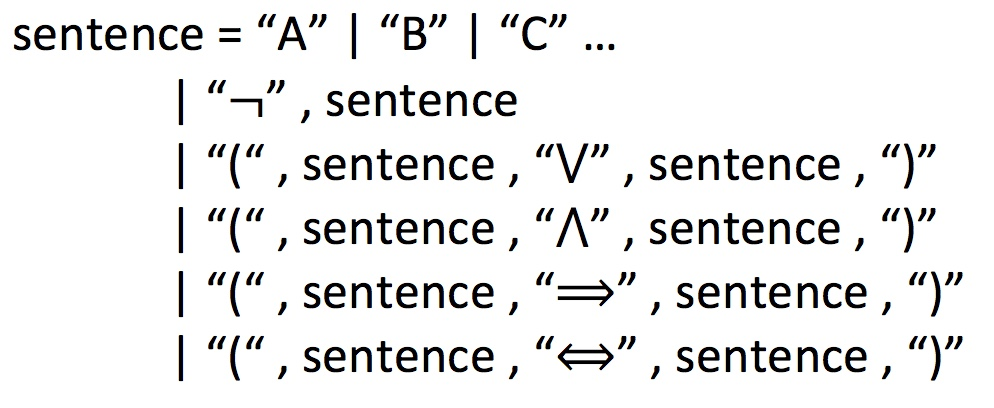
\includegraphics[width=100mm]{figures/PropositionalSentences}}
  \caption{Propositional Logic Grammar Rules}
\end{figure}

I have now defined a Propositional Logic language for this project. I have added brackets into the rules in order to ensure that it is possible to fully understand what a Propositional statement is saying and is therefore unambiguous. Without brackets some statements may become a bit ambiguous and difficult to understand. Truth tables can be used to interpret all of the possible results of a logical sentence. This helps users to plan for any possible outcomes of a set of propositions occurring.

\pagebreak
\begin{exmp}Examples of Propositional Statements using our language
\begin{itemize}
\item A $\Rightarrow$ B
\item B $\wedge$ A
\item ((A $\Leftrightarrow$ B) $\vee$ C)
\item $\neg$A $\Rightarrow$ (B $\Rightarrow$ C)
\end{itemize}
\end{exmp}


\subsection{Predicate Logic \label{predicate}}
Propositional logic is very useful when trying to represent the truth values of propositions, but there is limited scope in this formalisation as to the type of statements that can be represented. For example if I wanted to represent the statement "some boys like football", it would be very difficult to do this using just Propositional Logic. This is why I decided to also check proofs of the more useful first order Predicate Logic. This logical system allows users to both apply properties to specific objects and add quantifiers to them. This makes it much more expressive and useful in real world applications. 

The properties that an object has are called a Predicate. Predicates can be unary where they have just one property, or they can be n-ary describing relationships between them and other predicates. Predicate logic also includes two quantifiers that allow this formalisation to be more expressive. The first quantifier is a "for all" quantifier ($\forall$). This enables the representation of statements like "all dragons are green". The other quantifier is the "exists" quantifier ($\exists$). This quantifier allows the representation of statements such as "some dragons are blue".These two quantifiers together, increase the expressive power that can be created using this logical system. Below are some examples of statements that can be created using Predicate logic.

\begin{exmp}Examples of Predicate Statements
\begin{itemize}
\item $\forall x.P(x)$
\item $\exists y.bird(y)$
\item $\forall y.dark(y) \Rightarrow hates(x,y)$
\end{itemize}
\end{exmp}

\subsection{Natural Deduction}

The logical systems that were introduced above present a language and an interpretation using Propositional and Predicate atoms. All the reasoning that can be taken away from these systems are based on truth tables. Truth tables are a way of considering all of the possible outcomes of a statement filled with atoms that can be true or false. For simple systems truth tables are enough to be able to prove and reason about a situation. In order to be able to consider much more complicated problems, the truth tables would need to be very large, making it a time consuming problem to solve. It is therefore, necessary to introduce a formal system which provides the tools to solve and deduce these problems. To solve this problem Natural Deduction was created. Using a set of strict rules, Natural Deduction allows the deduction of the consequences of any Propositional or Predicate statements that are given, showing the immediate outcome. This apparatus is very useful in solving logical problems in all areas. When a statement can be deduced from a number of premises using Natural Deduction it is placed on the right side of a $\vdash$ symbol, while the original premises will be listed on the left of this symbol. Natural Deduction has a list of rules for both Propositional and Predicate logic allowing the deduction of the consequences of any premise. This proof solving methodology can also be used to solve proofs with no premises using its complex rule-set.

There are ten Propositional rules for Natural Deduction that can be used to form proofs (see Appendix \ref{appendix:nd-prop}). In this report I have outlined the rules based on the following process. Each rule consists of a horizontal line with the resulting expression or expressions placed beneath it. The expressions are either assumptions (where indicated) or expressions that need to be derived in order for the result below the line to be proven. For example, in the case of "And Introduction", both A and B need to be derived in order for the introduction to come into effect. In several cases, such as "Implies Introduction", an assumption must be made and a sub-goal proven in order for the expression below the line to be proven. These rules can be combined together to make-up complex Natural Deduction proofs.

\subsubsection{Propositional Rules Examples}

Throughout this project I have used the Gentzen Natural Deduction system. This means that I have set out the proofs as shown in the examples below. The first example shows a basic proof with the given premise written first followed by the various deductions made throughout the proof. On each line of the proof, I have written a justification of the rule that was used together with the lines that the rule has used to make the deduction.

\begin{exmp} Show that $A \wedge B \vdash A \vee B$

\begin{fitch}
\fj A \wedge B & Given \\
\fa A & $\wedge$-Elim (1) \\
\fa A \vee B & $\vee$-Intro (2) \\
\end{fitch}

\end{exmp}

The next two examples require an assumption to be made at some point in the proof that will allow the user to deduce their required outcome. Throughout this project when an assumption occurs in a proof I have highlighted the assumption and its result by formatting it slightly to the right of the rest of the proof. This makes it stand out and more readable for the user, alerting them to the new scope that has been entered.

\begin{exmp} Show that $ A \Rightarrow B \vdash \neg (A \wedge \neg B)$

\begin{fitch}
\fj A \Rightarrow B & Given \\
\fr \fa A \wedge \neg B & Assumption \\
\fa \fa A & $\wedge$-Elim (2) \\
\fa \fa B  & $\Rightarrow$-Elim (1) \\
\fa \fa \neg B & $\wedge$-Elim (2) \\
\fa \fa \bot & $\neg$-Elim (4,5) \\
\fa \neg (A \wedge \neg B) & $\neg$-Intro (2,6)
\end{fitch}

\end{exmp}

\begin{exmp} Show that $A \Rightarrow B, B \Rightarrow C \vdash A \Rightarrow C$

\begin{fitch}
\fa A \Rightarrow B & Given \\
\fj B \Rightarrow C & Given\\
\fr \fa A & Assumption \\
\fa \fa B & $\Rightarrow$-Elim (1,3) \\
\fa \fa C & $\Rightarrow$-Elim (2,4) \\
\fa A \Rightarrow C & $\Rightarrow$-Intro (3-5)
\end{fitch}

\end{exmp}

\pagebreak
\begin{exmp} Show that $A, A \Leftrightarrow B \vdash B$

\begin{fitch}
\fa A &  Given\\
\fj A \Leftrightarrow B & Given \\
\fa A \Rightarrow B & $\Leftrightarrow$-Elim (2) \\
\fa B & $\Rightarrow$-Elim (1,3) \\
\end{fitch}

\end{exmp}

The next example shows a proof which contains no premises but only the resulting expression. Several assumptions therefore have to be made using the Natural Deduction rules in order to solve this proof.

\begin{exmp} Show that $\vdash A \vee \neg A$
	
	\begin{fitch}
	
		\fr \fa \neg (A \vee \neg A) & Assumption \\
		\fr \fa \fa A & Assumption \\
		\fa \fa \fa A \vee \neg A & $\vee$-Intro (2) \\
		\fa \fa \fa \bot & $\neg$-Elim (1,3) \\
		\fa \fa \neg A & $\neg$-Intro (2,4)\\
		\fa \fa A \vee \neg A & $\vee$-Intro (5) \\
		\fa \fa \bot & $\neg$-Elim (1,6) \\
		\fa \neg \neg (A \vee \neg A) & $\neg$-Intro (1,7) \\
		\fa A \vee \neg A & $\neg \neg$-Elim (8)
	\end{fitch}
	
\end{exmp}

Although it is not an official rule, I have implemented an additional rule of availability to this project. This rule uses an already proven expression later on in the proof, in order to meet the desired outcome. This rule helps to keep proofs concise and readable, especially when it comes to more complex proofs. An example of how this rule is used can be seen in the example below:

\begin{exmp} Show that $B \vdash A \Rightarrow B$
	
	\begin{fitch}
		\fj B & Given \\
		\fr \fa A & Assumption \\
		\fa \fa B & Available (1) \\
		\fa A \Rightarrow B & $\Rightarrow$-Intro (2,3) \\
	\end{fitch}
	
\end{exmp}


\subsubsection{Predicate Rules Examples}

In Predicate Logic, similar Natural Deduction proofs can be created. These proofs, as well as using the Propositional rules, have their own set of rules (see Appendix \ref{appendix:nd-pred}) that the user can use to form a proof. This means that very complex proofs can be created. Below are some examples of what these proofs may look like.

\begin{exmp} Show that $P(m),  \forall x.(P(x) \Rightarrow Q(x)) \vdash Q(m)$

\begin{fitch}
\fa \forall x.(P(x) \Rightarrow Q(x)) & Given\\
\fj P(m) & Given\\
\fa P(m) \Rightarrow Q(m) & $\forall$-Elim (1) \\
\fa Q(m) & $\Rightarrow$-Elim (2,3) \\
\end{fitch}

\end{exmp}

\begin{exmp} Show that $\forall x. \forall y.P(x,y) \Rightarrow \neg P(y,x) \vdash \forall x.\neg P(x,x)$

\begin{fitch}
\fj \forall x. \forall y.P(x,y) \Rightarrow \neg P(y,x) & Given\\
\fa \forall y. P(a,y) \Rightarrow \neg P(y,a) & $\forall$-Elim (1) \\
\fa P(a,a) \Rightarrow \neg P(a,a) & $\forall$-Elim (2) \\
\fr \fa P(a,a) & Assumption \\
\fa \fa \neg P(a,a) & $\Rightarrow$-Elim (3,4) \\
\fa \fa \bot & $\neg$-Elim (4,5) \\
\fa \neg P(a,a) & $\neg$-Intro (4,5) \\
\fa \forall x.\neg P(x,x) & $\forall$-Intro (6)
\end{fitch}

\end{exmp}

\begin{exmp} Show that $s=t \vdash (s = u) \Rightarrow (t = u)$

\begin{fitch}
\fj s = t & Given\\
\fr \fa s = u & Assumption \\
\fa \fa t = u & Substitution (1,2) \\
\fa (s = u) \Rightarrow (t = u) & $\Rightarrow$-Intro (2,3) \\

\end{fitch}

\end{exmp}
\pagebreak

\section{Design \label{design}}

The design methodology that I decided to use for this project is the Model View Controller architecture. This entails the separation of the front-end website components from the back-end where the actual core functionality of the system is written. These two areas are then controlled by various controller classes, which bring all of these components together to create the finished application. I chose this methodology in order to make the system easier to understand and later build on. Whenever I need to add an extra feature to the application, I am able to just update the model part of the code-base and then change the front-end view code. This is much simpler than having all of the code together in one large code base. This methodology therefore made the development of this application much easier.


\subsection{Model}
The model part of any Model View Controller structured project, controls the main pieces of functionality of the application. This is, therefore, the part of the code-base that actually creates the problem solving features needed by the user. In order to create the functionality required for me to meet my objectives, I had to devise a fitting back-end design. There are lots of different problems that needed solving, so I tried to separate the different parts of my code-base into obvious classes that would make the code easy to read by any third party.

\subsubsection{Component}
In both Propositional and First Order Predicate logics, logical expressions can be made up of two different components, Propositions (or Predicates for Predicate logic) and Operators. For this project both of these components require some common functionality such as how they are converted to Strings, how they are interpreted when input by the user and how equality between them is worked out. Due to this common functionality I decided to create an interface called Component which encompasses all the commonly used methods used by each of these components. I then created a Proposition and an Operator class which would each represent a component type. Each of these classes would inherit from the Component interface. This setup was very useful in other parts of the code-base, as it allowed me to pass in a Component and then check which type of component I was dealing with.  

The Proposition class, as well as inheriting and implementing the common toString and equals methods from the Components interface, contained functionality to set and retrieve the name of a Proposition. A Proposition is made up of a String field which represents the name of the Proposition. This is one of the main components of expressions that are used in this logical system.

The Operator class is used to represent one of the seven operators used in this logical system, as described in the Background section above (see \ref{Background}). This class also inherits the toString and equals methods from Components, making it much easier to use when building expressions. Each Operator object is made of a string which represents its name and an enum value corresponding to each operator. I have created an enum called OperatorType, which contains all of the different operator types used in this logical environment. The reason that I set operators up in this way is that it easily allows me to check which operator is being used in an expression at any time due to its uniquely identified enum value. The rest of this class is filled with getters and setters that help with the general functionality of this logical system. The diagram below shows the class structure of the various types of Components.

\begin{figure}[!ht]
	\centering
	\makebox[\textwidth]{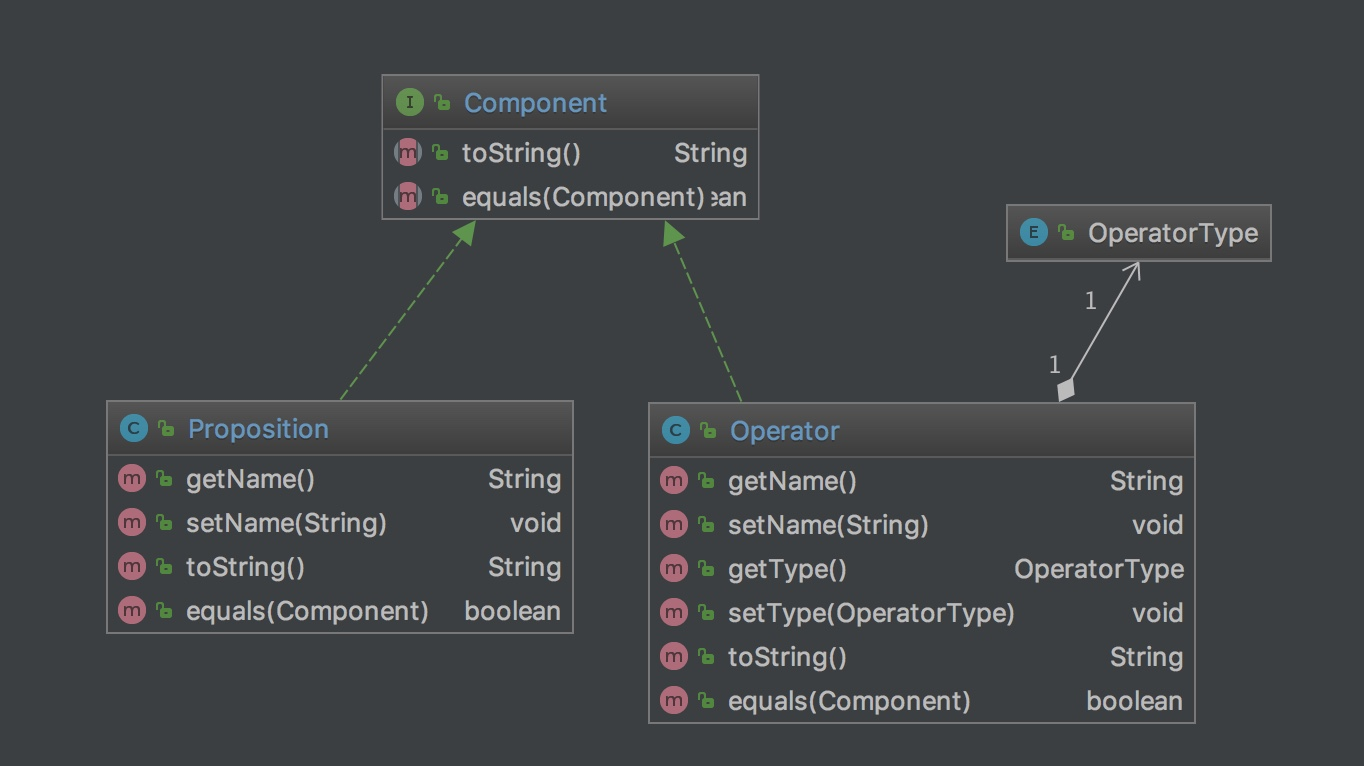
\includegraphics[width=\linewidth]{figures/ComponentsUML}}
	\caption{Component class structure}
\end{figure}

\subsubsection{Expression}

When using Natural Deduction, a proof is represented by a set of expressions each derived from previous expressions based on the Natural Deduction rule-set (see Appendix \ref{appendix:nd}). Expressions are therefore a fundamental building block of proofs. I created an Expression class, inside which I represented an expression itself by a list of Components. An Expression object has several other properties which are very helpful when functionality is applied to them. Each Expression keeps track of which line it represents in a proof, a very useful feature when applying rules that depend on several different lines in a proof. Using an enum which enumerates all of the different Natural Deduction rules that can be applied, each Expression also stores the rule that was used to derive it. This makes it simple to find out which rule was used when an Expression was formed, and is especially useful when carrying out the proof validity checking process.

The most important operation that the Expression functionality carries out, is the parsing of expressions from their String inputs. It is at this stage of the process that the Components themselves are checked to be valid and if so are added to the Expression list. If any Components or the Expression as a whole are not valid, the entire process will be halted and the user alerted. This process enables the creation of an internal representation of the expression, making it easier to use when applying the various types of functionality later on in the programme. In order to effectively carry out the creation of this internal representation, and to help with the various operations that are carried out on expressions, a lot of extra functionality has been added to Expressions. Functionality such as equality and splitting Expressions around an Operator among others, have been added as they are very useful when applying the various Natural Deduction rules to an expression, especially for elimination rules which require an expression to be split into one or two sub-expressions around the specified operator. An Expression object is, therefore, a fundamental building block for logical proofs in this project.

\subsubsection{Proof}

In order to represent the proofs that the user inputs into the system, I created a Proof class. This class contains a large amount of functionality used to represent these proofs in a way that they can be manipulated to help solve Natural Deduction proofs. In this class a proof is represented by a list of expressions, each representing a line in the proof. 

Each Proof object contains functionality that reads in Expressions along with their associated rules, and stores them in a list representing the proof. Proofs also provide a large amount of functionality that checks whether each of the Natural Deduction rules have been applied correctly.  For example if an expression was created using And Introduction, the code would check to ensure that both the right and left hand sides of the And operator have been proven earlier on in the code. If a rule has been used incorrectly, or cannot be used at this stage in the proof, then a rule error will be thrown aborting this entire process. These checks are a fundamental part of this tool as they are what alerts the user as to whether their proof is valid. 

Another additional complexity that has to be taken into account when forming Proofs, is the scope that the current expression is in. Whenever an assumption is made a new scope (or box), is opened until it is closed by certain rules being completed. Once this has happened nothing after this scope can use any expressions inside this scope for any further steps of the proof (apart from the result of the scope). This is another check that the code must make when assessing whether a rule has been used correctly at any point of the proof. I implemented this checking functionality by creating a list which, before starting the process of checking whether rules have been used validly, stores as pairs the starting and ending indexes of boxes in the proof. Then as each rule is checked to see whether it is valid, the referenced line indexes for the rule are checked to see whether they fall within a completed box before the current expression in the proof. If they do, this check fails and an associated error is generated. This mechanism ensures that only references that are in-scope can be used to create new lines in the Proof. This Proof object, therefore, is the basis that most of the applications core functionality is built on.

\subsubsection{Error Checking}

One of the main goals that I set at the beginning of this project, was to make a Natural Deduction solver which is a tool that can help teach people how to successfully solve these types of problems. I therefore made sure to have a very detailed error message system that allows a user to see exactly where they have gone wrong. This would mean that they can learn from any mistakes that they may have made. In order to make this as easy as possible, every error message that is displayed contains the type of error that has occurred, the line that it was thrown on as well as some extra information about the associated problem. This makes it very easy for the user to immediately understand what they have done wrong. In the case where no errors are thrown, the programme will display the string "Proof is Valid", alerting the user to their valid proof. 

The first type of error check that occurs as soon as the parser starts to read the user input, is for Syntax errors. This check ensures that as Components are added only valid expressions are formed.  For example if two operators are added to an expression in a row, this error will be thrown. Similarly, if there are any mismatched brackets in an expression, a syntax error will immediately be thrown. This type of error is fundamental as the syntax of the proof must be completely correct in order for the user to move onto actually solving the proof at hand. This check is done right at the beginning of the parsing process for this very reason.

The other type of error check, which helps to make this an educational tool, is for Rule errors. Whenever a proof is entered by a user, there is a function in the Proof class which goes through the proof and ensures that each line is valid. It does this by going through the list of expressions (the proof), and checks whether the specified rule can be used in the proof at this point. It also checks that the lines referenced by this rule are valid and are not out of scope. If all of the rules used are used correctly then the user is notified that the proof is completely valid. If not, the user will be alerted to the line and rule which was incorrectly used, helping them to learn from their mistake. In order to clearly show the user all of the rules that have been broken at the same time, the Proof class contains an error list. This list slowly builds up as the proof is checked, and is then displayed after this process is complete. I decided to allow this accumulation of errors so that a user can fix several errors that exist at a time, rather than having to solve several over a long chain of trial and error. These error checks are done after any syntax errors, that may cause expressions to be invalid, have been fixed.

\subsubsection{Workflow}
Up to this point, I have explained the core features that this application's functionality is built from. It is upon these features that further, more complex additions are made to this software. In this section, I briefly describe the overall workflow process, from user input all the way to the output that they ultimately receive.

The user starts off by inserting two strings into the core functionality, each separated by a newline character for each line in the proof. The first string represents the various expressions that make up the proof, while the second represents the associated rules used to form each expression. Once the user has entered these two strings they are able to submit their proof to check whether it is valid. Before doing this they have the option of applying other further functionality such as a validity check or turn on hints, as discussed in the next two sections.

Once the user has submitted the proof, a Proof object is created for this proof and the strings are tokenised by new-lines. For each line of the proof an Expression object is then created containing the expression itself as well as the associated rule that was used to create it. The line numbers of any lines in the proof that are referenced in order for a rule to be applied, are also added to this newly created expression. In order to create these expressions, each Expression takes the string representing the expression itself and tokenises it by spaces. At this point the tokens are checked to see whether any Syntax errors exist and if so the entire process will be terminated and the user alerted. Assuming no Syntax errors are thrown, each token is then converted into a Component depending on its type. Each of these Components are then added to the list representing the expression. After each Expression has been created, they are all added to the list of expressions stored in the Proof object. The application now has an internal representation of the users proof.

Now that a Proof has been created, the functionality begins to check whether the various rules have been applied correctly throughout the proof. It does this by iterating through the list of expressions from the bottom up checking each rule as it passes. Within each rule check, the reference or references quoted are checked to ensure that they are in scope, and that they are valid references to use for the associated rule. The system also checks whether the correct number of lines have been referenced in order for the rule to be successfully applied. If any of these checks fail, an associated Rule error will be thrown terminating the entire process and alerting the user. If all of the rules used are checked and proven to be valid, the system concludes that the proof as a whole is valid. If this is the case, the user is alerted to this fact through a display of "Proof is Valid" on the screen. This ends the workflow of this application as it checks a proof for any errors a user may have included in their Natural Deduction proofs. 

\subsubsection{Validity Checking \label{validity}}
Natural Deduction proofs can be quite long, adding an extra difficulty when trying to debug a mistake that was made in a proof. When solving a proof, it would be helpful to know that you can solve the proof with the given premises and result at all. It would be pointless to just start solving the proof if you will never reach the resulting expression. This is a major problem faced by even the more experienced solvers of these problems.

In order to remedy this potential issue I have added an optional extra validation stage before the main solver functionality. This stage allows the user to input their desired premises and result, and they will be used to check whether a proof using these expressions is valid. In order to implement this I have used the Truth Table validation method. This works by calculating the truth values of each premise and the result. The method then looks to see whether in the cases where all of the premises evaluate to true, the result expression also evaluates to true. If every case of the premises all evaluate to true, then we know that the proof is valid and that there is a possible proof that can be used to solve it. I implemented this check by first creating a TruthTable object, which is represented by a 2D array. When the user submits their premises and result, this array is populated with the possible input values for each proposition, the truth values of each premise in each of the cases, and the truth value of the result in each case. This object then has functionality that checks whether all of the truth values evaluate to true in the required cases, and if so designates this proof as valid. This whole mechanism will save a user a lot of time by allowing them to see immediately whether a proof they are about to try to solve is solvable. Although this algorithm is relatively efficient for small expressions, this algorithm does not scale very well and would be very inefficient for large expressions. However, for use as a Natural Deduction solver where most expressions will have less than a dozen propositions, this does not present a problem. This is why I chose to use this algorithm to validate proofs. 

\subsubsection{Hints \label{hints}}

One of the advanced features that I set out to implement during this project is hints. I wanted to allow a user to start a proof and if they become stuck at any step, they could use my software to gain a hint as to what rule to apply next. This feature is something that is lacking in similar software such as Pandora. When first planning to include this feature in the project,  I felt that I would start by implementing a simple form of hints, where when a hint was requested I would try each of the rules and reply to the user with any rules that didn't throw any errors. Obviously, this is quite a short-sighted way of implementing this, as a user could be sent off in a completely wrong direction. Also, when it comes to introduction rules, there can be quite a lot of different possible cases to consider. I therefore decided that this methodology for generating hints is not useful for a user and started to explore some alternative methods.

Based on this exploration, I decided that the best way to implement this feature would be to actually apply an algorithm which solves the proof first. This would mean that when a hint is requested the system compares the users proof so far to the solved proof, in order to generate a hint for the next step. The first algorithm that I tried was one which took the premises that were given by the user and firstly tries each of the elimination rules on them several times. As this was happening the algorithm built up a list of possible proofs based on the steps found to be valid so far. The algorithm then tried some introduction rules in order to move further into the proof. This process would continue in a loop until either the resulting expression was reached, or a time-out was met. 

Although this algorithm was able to solve the proofs in order for hints to be generated, in proofs which include any introduction rules, the algorithm took quite a long time and in some cases failed completely. This is due to the large number of options that needed to be tried for each introduction rule, adding even more possible combinations to the list of possible proofs. This is especially true in the case of "Or Introduction" where there are so many possible expressions that can be created. Almost anything can be added to one side of an expression using this rule, leading to the list of possible proofs growing quickly. It is also not guaranteed that the required expression will ever be found. For example, if one was given the expression "A" and wanted to prove as a resulting expression "A | Q". This algorithm will keep trying to find a fitting right hand side of the expression, but may never find one, or if it does, only after a large amount of time. This case and others showed me that in order to be able to effectively solve any Natural Deduction proof problem, I would have to take the results and sub-results into account throughout the solving process. For example in the case mentioned above, the algorithm should see "A | Q" and know when applying "Or Introduction" to try using the Proposition "Q". Similar problems to this occur when using the other introduction rules making this algorithm very unreliable. Therefore, I decided to search for some more efficient algorithms that take this idea into account to use to solve these problems.

After further research of this topic, I found a resource containing a proof solving algorithm that could easily be adapted to use in this tool in a paper called Automated First Order Natural Deduction \cite{ndAlgo}.  This algorithm works in a completely different way to the one I devised above as it actually takes into account the goals and sub-goals of the proof. Using two lists, the algorithm keeps track of the current state of the proof, which is initially just the premises, and of the current sub-goal that the algorithm is trying to achieve, which is initially the resulting expression. As the algorithm proceeds new sub-goals are added to the list of goals in order to direct the proof towards its ultimate resulting goal. Both lists are expanded using the Natural Deduction rules until one of the premises can be unified with one of the goals. If this is the case that goal will be removed from this list. Eventually the resulting goal will be unified and the algorithm will terminate. The rules that are applied at each step are dependent on the structure of the expressions in the proof so far. Elimination rules are applied first and as a last resort an introduction rule will be applied. This algorithm has been proven to always terminate if a valid proof has been given. A summary of exactly how this algorithm functions can be seen in Algorithm \ref{solveAlgo}. The main benefit of this algorithm, is that by setting up sub-goals, the algorithm does not have to spend large amounts of time looking for possible combinations of expressions for introduction rules. Rather it takes into account the goals of the introduction rules and will apply the appropriate rules in order to meet it. This algorithm therefore works relatively efficiently in all cases and can scale very well. This makes this algorithm much better for my purposes and is why I chose to use it for this part of LogicAssistant's functionality. 

\begin{algorithm} \label{solveAlgo}
	\caption{Automated First Order Natural Deduction Proof Solver (my implementation based on~\cite{ndAlgo})}\label{euclid}
		\noindent\makebox[\textwidth][c]{%
		\begin{minipage}{.92\linewidth}
		In this algorithm I represent a proof as $P \vdash G$, where the set \textit{P} are the premises and \textit{G} is a set containing the goal of the proof together with any sub-goals. The two lists used in the algorithm are \textit{list\_proof}, to store the current state of the proof and \textit{list\_goal}, to store the current goals and sub-goals of the proof. $G_{n}$ will also be used to keep track of the current goal. Reachability of the current goal shows whether an expression is in scope and can therefore be accessed at a stage in the proof.
		
			\begin{enumerate}
				\item Given the problem $P \vdash G$, take \textit{G} as the initial goal, add it to \textit{list\_goals} and set the current goal equal to \textit{G}. If the set \textit{P} is not empty then add \textit{P} to \textit{list\_proof}.
				
				\item 
				\begin{enumerate}
					\item If $G_{n}$ has been reached go to step 3
					\item If Elimination rules are applicable go to step 4
					\item If no more Elimination rules are applicable go to step 5
				\end{enumerate}
			
				\item 
				\begin{enumerate}
					\item If $G_{n}$ is the initial goal then terminate as the proof has been found
					\item Based on the structure of $G_{n}$, invoke Introduction rules, then go to step 2
				\end{enumerate}
				
				\item Invoke Elimination rules, then go to step 2
				
				\item Create a new goal that will help to achieve the current goal, set $G_{n}$ to this goal and add it to \textit{list\_goals}
				\begin{enumerate}
					\item Analyse the structure of $G_{n}$ and add appropriate assumptions or sub-goals to the lists based on the definitions below (note: some rules are defined differently to  \cite{ndAlgo}):
					
					Let $P_{1}$ ... $P_{k}$ = $\Gamma$, $G_{1}$ ... $G_{k}$ = $\Delta$ and $F$ is an elementary formula:
				
					\vspace{0.15cm}
					\noindent\makebox[\textwidth][c]{%
						
					\begin{minipage}{.92\linewidth}
						
					
						$\Gamma \vdash \Delta, A \Rightarrow B$   \hspace{1cm} $\xrightarrow{\makebox[1cm]{}}$  \hspace{1cm} $\Gamma, A \vdash \Delta, A \Rightarrow B, B$
						
						$\Gamma \vdash \Delta, \neg A$   \hspace{1.6cm} $\xrightarrow{\makebox[1cm]{}}$  \hspace{1cm} $\Gamma, A \vdash \Delta, \neg A, \bot$
						
						$\Gamma \vdash \Delta, A \wedge B$   \hspace{1.15cm} $\xrightarrow{\makebox[1cm]{}}$  \hspace{1cm} $\Gamma \vdash \Delta, A \wedge B, B, A$
						
						$\Gamma \vdash \Delta, A \vee B$   \hspace{1.15cm} $\xrightarrow{\makebox[1cm]{}}$  \hspace{1cm} $\Gamma \vdash \Delta, A \vee B, A$
						
						$\Gamma \vdash \Delta, A \vee B$   \hspace{1.28cm} $\xrightarrow{\makebox[1cm]{}}$  \hspace{1cm} $\Gamma \vdash \Delta, A \vee B, B$ (if above rule fails)
						
						$\Gamma \vdash \Delta, A \Leftrightarrow B$   \hspace{1cm} $\xrightarrow{\makebox[1cm]{}}$  \hspace{1cm} $\Gamma \vdash \Delta, A \Leftrightarrow B, A \Rightarrow B, B \Rightarrow A$
						
						$\Gamma \vdash \Delta, F$   \hspace{1.82cm} $\xrightarrow{\makebox[1cm]{}}$  \hspace{1cm} $\Gamma, \neg F \vdash \Delta, F, \bot$
						
						$\Gamma, \neg A \vdash \Delta, \bot$   \hspace{1.155cm} $\xrightarrow{\makebox[1cm]{}}$  \hspace{1cm} $\Gamma, \neg A \vdash \Delta, \bot, A$
						
				\end{minipage}}	
			\vspace{0.15cm}
			
						For "Or Elimination", I treat this rule in the same way as the introduction rules, so both of the next two rules must be applied:
						\vspace{0.15cm}
						
						\noindent\makebox[\textwidth][c]{%
							
							\begin{minipage}{.92\linewidth}
						$\Gamma, A \vee B \vdash \Delta, C$   \hspace{0.75cm} $\xrightarrow{\makebox[1cm]{}}$  \hspace{1cm} $\Gamma, A \vee B, A \vdash \Delta, C$
						
						$\Gamma, A \vee B \vdash \Delta, C$   \hspace{0.75cm} $\xrightarrow{\makebox[1cm]{}}$  \hspace{1cm} $\Gamma, A \vee B, B \vdash \Delta, C$
						
								\end{minipage}}	
						
						 \vspace{0.15cm}
			
					then go to step 2
					\item If all formulae in \textit{list\_proof} have been considered as sources for new goals (based on rules in (a)), terminate the algorithm as no proof has been found
				\end{enumerate}
			
				
			\end{enumerate}
		
		\end{minipage}}

\end{algorithm}


In addition to the basic algorithm, I added a few features to optimise the speed that the algorithm runs at. In particular, at the start of the algorithm I added a check which looks at the resulting expression of the proof and sees from the start whether it contains an implication operator or starts with a not operator. If so, then the algorithm now knows that the last rule applied will either be "Implies Introduction" or "Not Introduction". The algorithm can therefore skip the elimination rule checks at the beginning and go straight to these introductions. This speeds up the whole process in these cases significantly and ensures that the proof is as concise as possible. An example of this could be when solving a proof with premises "B" and "$D \wedge E$" and desired result "$A \Rightarrow B$". Without my optimisation the proof would start off with the "And Elimination" of "$D \wedge E$", a completely unnecessary step. This just makes the proof longer. With my extension immediately the algorithm will see the $\Rightarrow$ in the result and will add an assumption of "A", thereby not wasting any time trying any elimination rules. My optimisation works similarly for results beginning with a not operator. This extension clearly speeds up the algorithm's overall running time and removes unnecessary steps from the proofs.

 The paper where I sourced this algorithm, defines its "Or Elimination" rule slightly differently to how I have in this project. In order to carry out an "Or Elimination", I split the two sides of the Or operator into two separate boxes and try to find the same resulting expression in each, thereby eliminating the original expression (rule taken from \cite{ndBook}). I therefore had to add some extra functionality for this case into the algorithm. I did this by first assuming the left hand side of the Or containing expression. I then created another temporary list to which I added the entirety of the proof so far, except that instead of assuming the left hand side expression, I assume the right hand side expression. The algorithm then continues, but whenever a new step is added to the main proof list, I attempt to add a new step to the temporary list. This continues until both lists reach the same expression. By implementing this rule in this way, I am able to use my definition for this rule whilst still benefiting from the use of this efficient algorithm. Using this algorithm I am able to solve any proof, and based on this provide the user with hints at any stage of a proof to help them learn how to solve Natural Deduction problems. 

In order to make this part of the software as useful to the user as possible, I decided to add two advanced extensions. Firstly, it is now not just at the end of a proof that a user can ask for a hint, but also in the middle. Sometimes when solving a natural deduction problem you can work out some sub-goals that will appear later on in the proof by working backwards from the goal. However, you may not be able to work out how to get to this sub-goal. In order to help combat this problem I have adapted the hint algorithm to allow the user to leave gaps in the middle of the proofs, and when the proof is submitted, hints will be generated to fill these gaps. An example of this can be seen in the following image typed into LogicAssistant.

\begin{figure}[!ht]
	\centering
	\makebox[\textwidth]{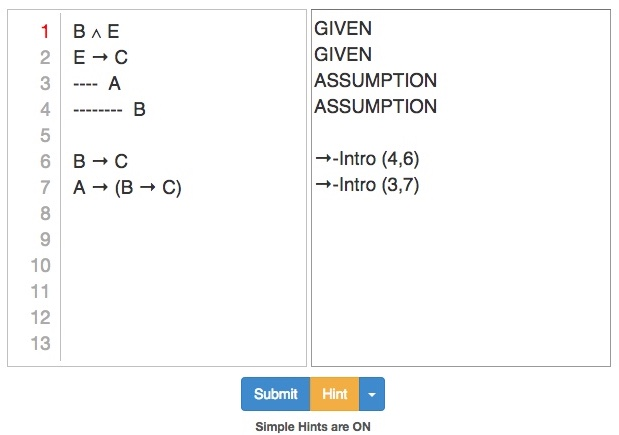
\includegraphics[width=13cm]{figures/hintInMiddle}}
	\caption{Example of hints in the middle of proofs}
\end{figure}

In this proof the user has been able to work out the first two steps, and has also been able to add a sub-goal as the second last step by working backwards. The user however does not know how to fill the gap that is left. By leaving a blank line, LogicAssistant will keep providing the user with hints until the proof has been completely solved. This feature is really important as a good technique to use when solving these proofs by hand is to work backwards, and now it is possible to continue using this method even when you get stuck midway. 

The second advanced feature that I have added is the tailoring of hints towards how the user has input the proof. Often there are multiple ways to solve a proof using Natural Deduction. The solving algorithm that this software uses tries to find the shortest optimal solution for these proofs, but that doesn't mean that other longer methods are invalid. As this is a learning tool, I decided that the hints generated should try to, where possible, follow the route that the user has started to take. Even if this means a longer proof, at least the user will be learning how to create valid proofs; the main objective of this tool. An example of this can be seen in the image below.

\begin{figure}[!ht]
	\centering
	\makebox[\textwidth]{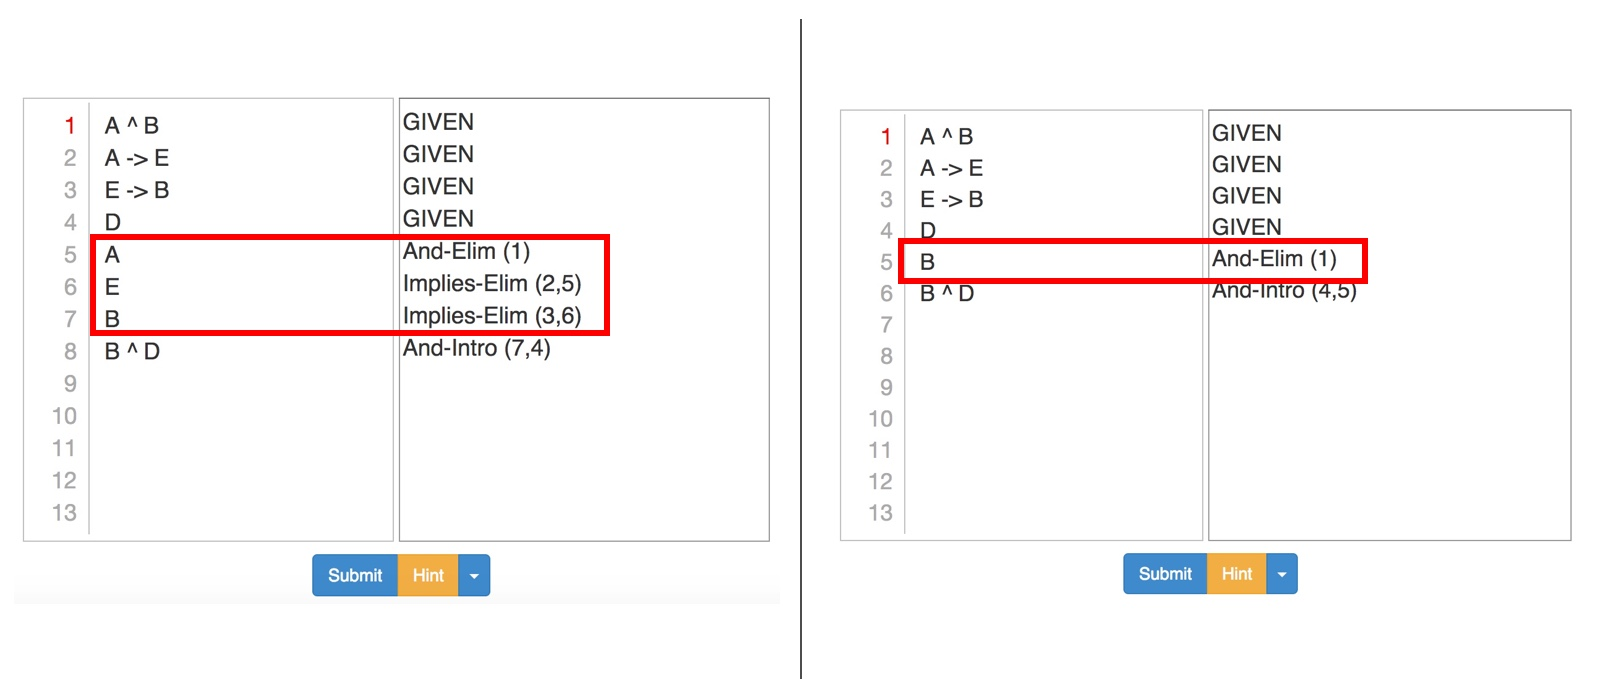
\includegraphics[width=\linewidth]{figures/proofComparison}}
	\caption{Comparison between possible proof make up}
\end{figure}

This example shows you two proofs with the same premises and goals, yet one is slightly longer than the other. The red boxes indicate the differences. Depending on which way the user takes, this algorithm will now learn from this and continue to follow in this direction. I was able to do this by, in step 1 of the algorithm (see \ref{solveAlgo}), when the premises and results are added to the two lists, also adding the steps of the proof that had already been entered by the user. This means that when the algorithm starts to run it continues on from where the user is up to, thereby helping to tailor the generated proof and hints to the users method. These two extra features together make this programme an invaluable tool when learning to solve these complex problems. 


\subsection{View}

\begin{figure}[!ht]
	\centering
	\makebox[\textwidth]{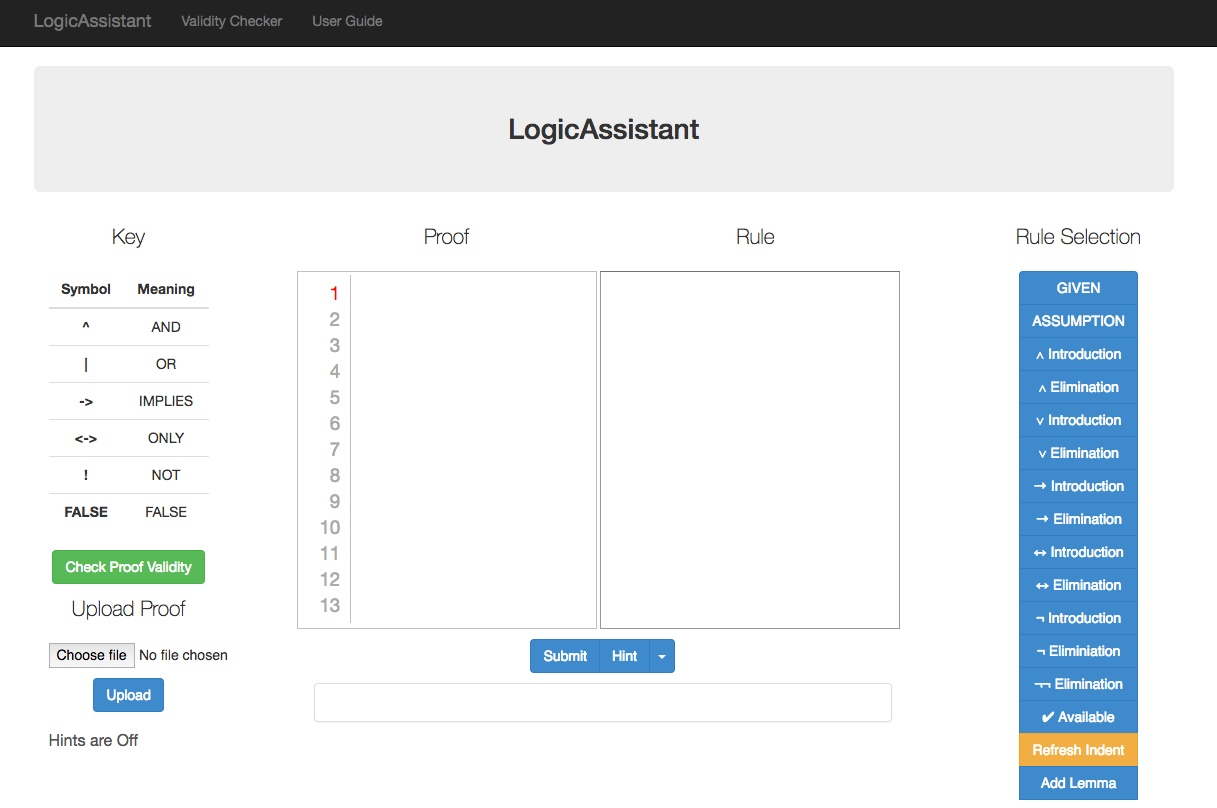
\includegraphics[width=13cm]{figures/wholePageImage}}
	\caption{Website homepage}
\end{figure}

One of the key components of this project is the design of the front-end. I wanted to make the application as easy-to-use and as appealing as possible to users looking for help in solving their Natural Deduction proofs. I therefore spent a long time perfecting this part of the application. As mentioned below (see \ref{JavaSpring}), I used Java Spring to create a front-end that uses the Java back-end of this project. This meant using Thymeleaf together with HTML and Javascript to create an easy to use, but powerful user interface. In order to perfect the website I carried out several iterations before deciding on this final design.



The website itself is made up of three pages. The first of which is the home page (see image above), which contains most of the core functionality of the application. This page is made up of several different components. When you load the page the first part you see is the two text areas right in the middle of the page. 

\begin{figure}[!ht]
	\centering
	\makebox[\textwidth]{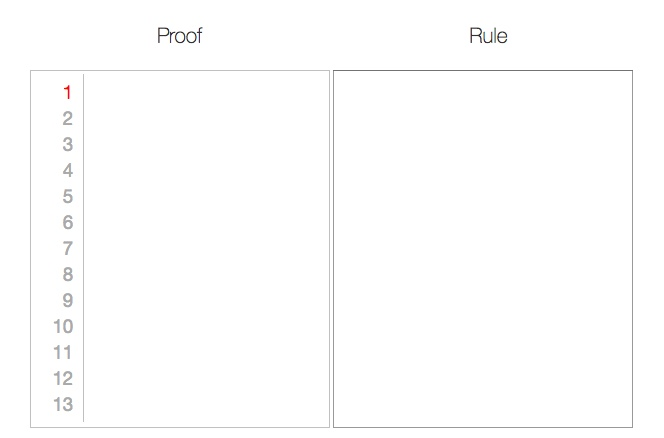
\includegraphics[width=13cm]{figures/textareas}}
	\caption{Proof input boxes}
\end{figure}


The left one includes line numbers and allows the user to type in each step of their proof. The text area on the right allows the user to add a rule for each line of their proof. A key is conveniently displayed on the left hand side of the page, to show the user how to represent each of the operators in this logical system. In order to insert a rule corresponding to a line in the proof, on the right hand side of the page there is a list of buttons each representing a different rule. When one is clicked on that rule is added to the next line of the proof. 

\begin{figure}[!ht]
	\centering
	\makebox[\textwidth]{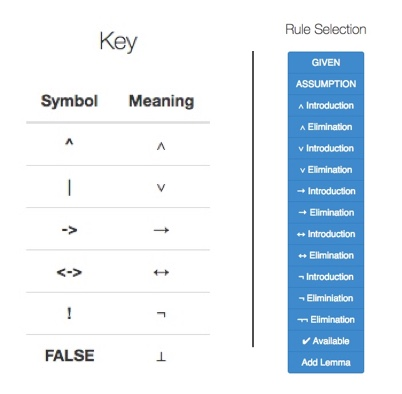
\includegraphics[width=10cm]{figures/key&rules}}
	\caption{Symbol Key \& Rule Buttons}
\end{figure}

If the rule needs references added to it regarding the lines in the proof it is using, the user can type these into the text area manually. If an assumption is used at any point of the proof, this left text area will automatically indent itself to represent any boxes (scopes) included in the proof. 

\begin{figure}[!ht]
	\centering
	\makebox[\textwidth]{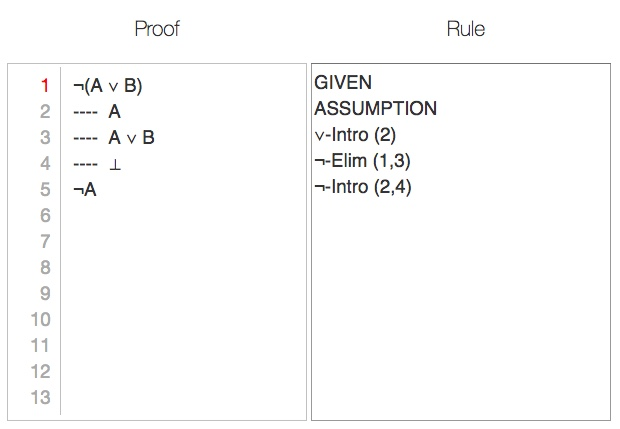
\includegraphics[width=13cm]{figures/indentation}}
	\caption{Full proof with references and indentation}
\end{figure}


Once the user has completed their proof they can click the submit button towards the bottom of the page, and the solver will alert them to whether their proof is valid. If not, it will display any syntax or rule errors, including some extra helpful information to assist them in solving any issues that may be present. 

\begin{figure}[!ht]
	\centering
	\makebox[\textwidth]{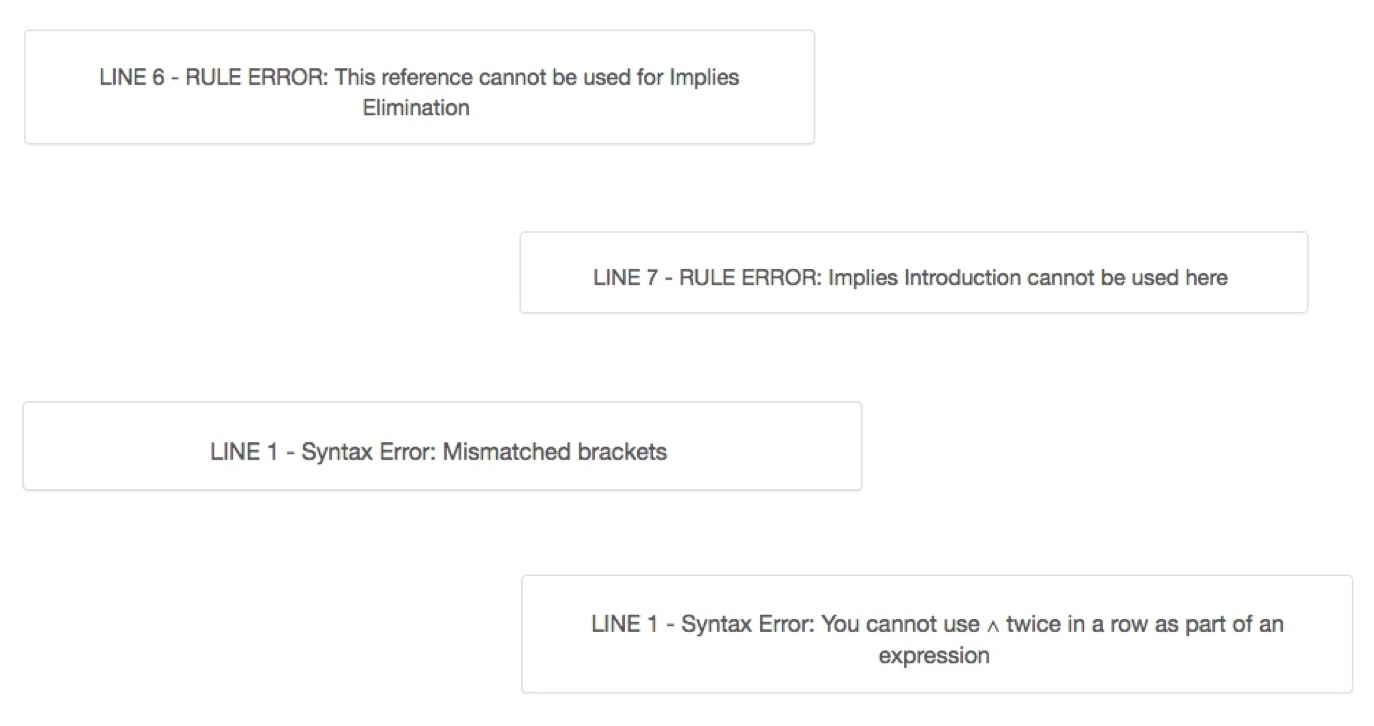
\includegraphics[width=13cm]{figures/errorsAndSubmit}}
	\caption{Error Message examples}
\end{figure}

If the user becomes stuck at any part of their proof, they can click the "Hint" button at the bottom of the page so that it turns orange. This means that basic hint mode has been turned on, so that when submit is now clicked, a hint will be delivered to the user in the output box at the bottom. If the hint button is used after the proof has already been solved, the user will be notified to this fact. Also, as mentioned above if the user has lines in the middle of the proof that they are stuck on, they can leave a blank line and an associated hint will be generated. All of these front-end features together make up the main functionality of this programme.
\pagebreak

\begin{figure}[!ht]
	\centering
	\makebox[\textwidth]{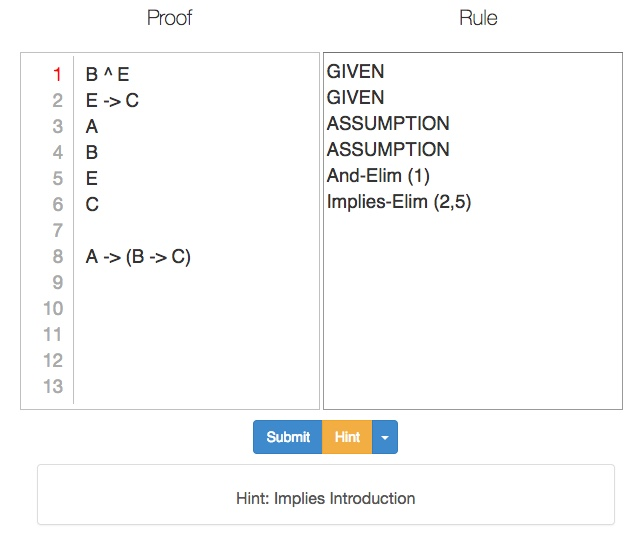
\includegraphics[width=13cm]{figures/hintProof}}
	\caption{Hint requested for a proof}
\end{figure}



This page also contains some other features that assist a user when using this software. Firstly, there is a drop-down menu towards the bottom of the page, that contains two useful options. An option to reset the page in order to type a new proof, and also a save proof as option. This allows the user to save any proofs they have, so that they can be revisited again on a later occasion. On the left hand side of the page there is also functionality that allows the user to upload their own proofs. This programme has its own file type (.la) and files of this type can be uploaded to this solver. The proof then can either be checked or added to and then saved again for future use. All of these small features together make using this system much simpler and straightforward for users to use.

\begin{figure}[!ht]
	\centering
	\makebox[\textwidth]{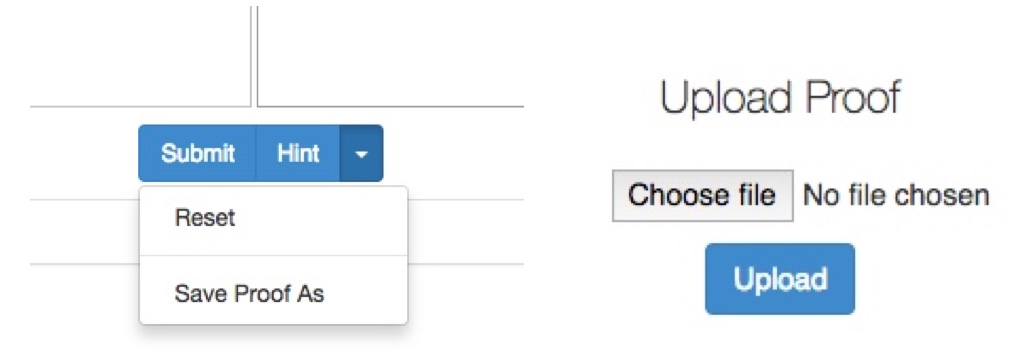
\includegraphics[width=13cm]{figures/extraFunctionality}}
	\caption{Additional Functionality}
\end{figure}



The next page of the web-app is the proof validation page. This can be accessed using a button on the left hand side of the home page. This page allows the user to type in their chosen premises and the resulting expression that they want to use in their proof. Then by clicking the "Check Validity" button, the validity algorithm will be triggered (see \ref{validity}), alerting the user as to whether the proof will be valid. This step saves the user a lot of time by allowing them to see whether the proof they are about to solve is solvable before they even start the proof solving process. Once this check has been completed the user can navigate back to the home page in order to actually solve their proof step by step.

\begin{figure}[!ht]
	\centering
	\makebox[\textwidth]{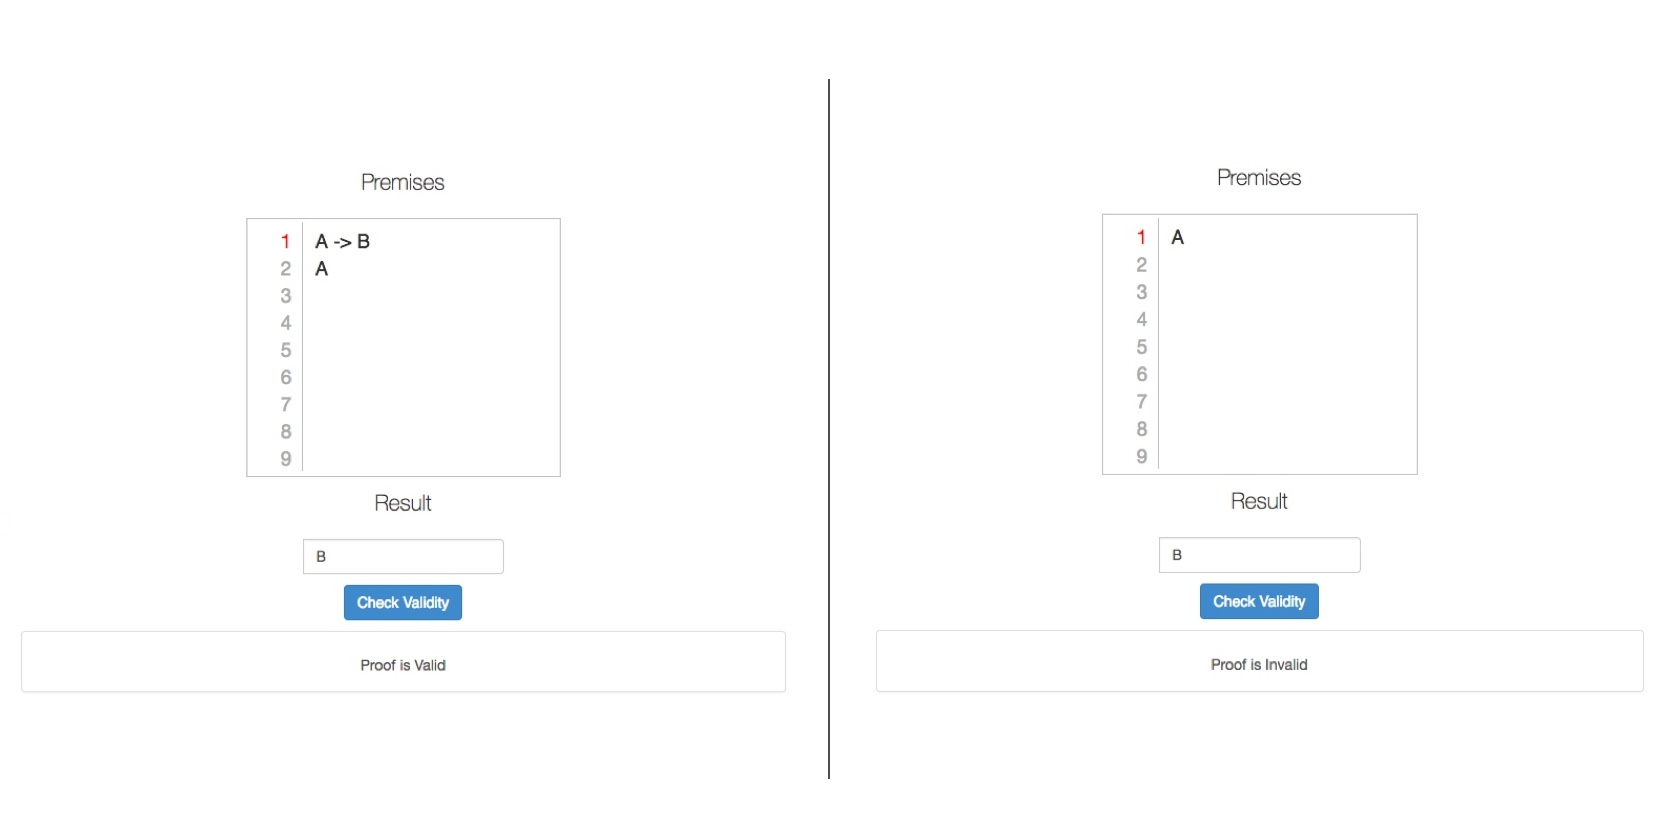
\includegraphics[width=\linewidth]{figures/validityChecker}}
	\caption{Validity Checker}
\end{figure}

The final and most important page of the application is the User Guide. This page contains a detailed description of how to use all of the features mentioned above. With the help of this page I believe that almost any user will be able to work out how to use most of the functionality on the website. In addition to this, throughout the website I have added tooltips onto some of the key pieces of functionality. This means that when a user puts their mouse over one of these tooltips they will be shown a small speech bubble explaining what that piece of functionality is used for. This will increase the ease at which new users are able to benefit from this software. This is therefore how the front end (or view) part of my application has been created.

\begin{figure}[!ht]
	\centering
	\makebox[\textwidth]{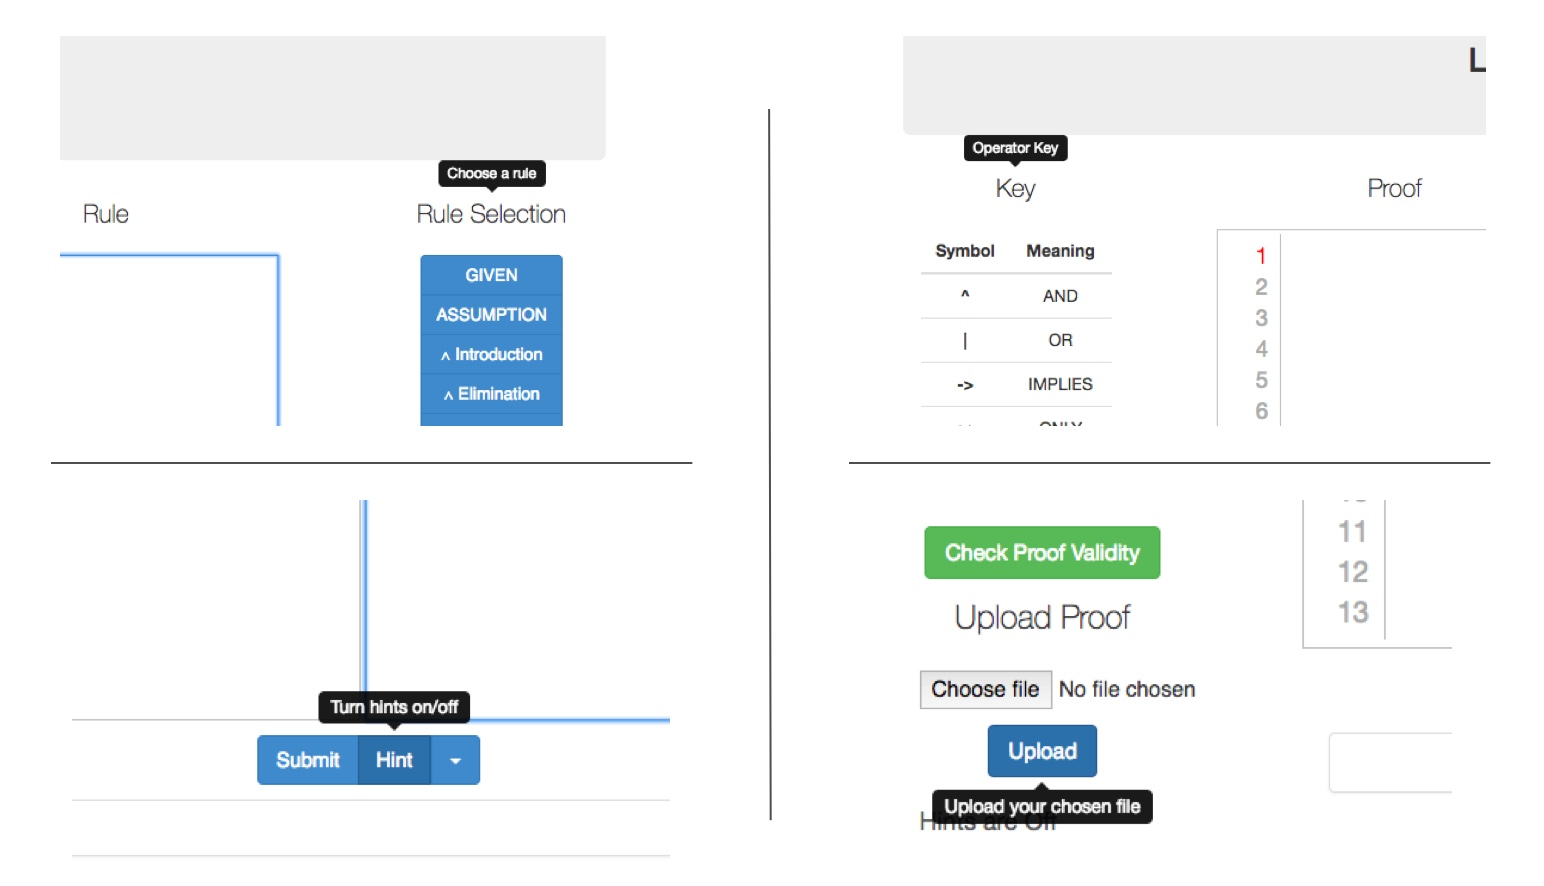
\includegraphics[width=\linewidth]{figures/tooltips}}
	\caption{Homepage Tooltips}
\end{figure}

\subsection{Controller}

In order to coordinate and control the model and view parts of this web-app, it was necessary to add some controller classes. As I used the Java Spring framework to build this application (see \ref{JavaSpring}), I was provided with some special controller functionality that can be used to control the entire programme. Therefore, each page has its own controller class which retrieves a mapping based on the url, and allows the passing of Java objects into the front end of the application. For example the main page receives a mapping of "/", as it is the home page, and the controller passes in a Proof object so that the associated functionality can be applied. This controller also has a post mapping which returns to this same page after the form has been submitted. Similarly, the validity page has its own controller which receives a mapping of "/validity" as the browser enters that page. The controller then provides a TruthTable object to the front end, so that it can be used to carry out the validation checks. These two controllers are therefore really important as they allow the various pages to communicate with each other, as well as to the back-end of the programme. This setup means that unlike Ajax, interactions are only made between the front-end and back-end on a page reloading. Although this led to a few complications, in the end I was able to connect all of the required components successfully. This therefore completes the setup of the Model View Controller infrastructure that I have built for this application.

\pagebreak

\section{Development Tools}

\subsection{Java}

When embarking on a project such as this, the language that is chosen to implement all of the complex functionality is very important. In particular the chosen language must be compatible with front-end infrastructures. Lots of languages also have extra features such as large testing frameworks and advanced IDE's that would make the whole process of making an application much easier. Also once a language has been chosen it would be a lot of work to then transfer to another language. I therefore spent quite a long period of time deciding which language was best suited for this project.

The first language that I considered using was Prolog. Prolog is already a language based on logical systems, and had I used it, representing logical statements would have been much simpler. I also found a user interface library that uses Prolog itself to create a front-end website for applications. Based on these finds I could have built this application using Prolog. The main drawback for me of using this language, is that I am not as familiar at using it as other languages, meaning that I would have to waste a lot of time learning the language first before actually starting the application. Also, some of the more advanced features that I wanted to add, such as hints, would have been quite hard to implement using this language. I therefore in the end decided to look at other languages to use for this project. 

The language I ended up settling on for this project was Java for a number of reasons. Firstly, Java is the language that I am most familiar with and I am able to use many of its advanced features and large array of libraries. This made it very easy for me to create the representation of Proofs, as well as some of the more advanced functionality for this project. Another reason that I chose to use Java is the number of libraries and data structures it offers. I was able to use advanced lists and hashMaps throughout the code in order to ensure that all of the required functionality worked as efficiently as possible. Other languages like Prolog do not have these resources. Java also supports the use of the JUnit library (see \ref{JUnit}), allowing me to ensure that all pieces of functionality are working as expected through the creation of a large test suite. On top of all of this, there are lots of tips and references available for the Java language for me to use whenever I needed them. In particular, the Java online community is much larger and more developed than Prolog's, which is a niche language only used for certain purposes. This meant it was easy for me to look up any problems I faced online. The only drawback that I found of using Java, is that it meant writing quite a large amount of code to create simple functionality, which can be quite time consuming. However, due to my knowledge of the language this did not hinder my progress too much. 


\subsection{Java Spring \label{JavaSpring}}

For this project, as I wanted to use Java to create the back-end functionality of the programme, I needed to find a framework that would make it easy for me to create a front-end that is compatible with this code. I also wanted to ensure that I was able to create a Model View Controller architecture (as argued in \ref{design}) for the code-base. I therefore decided to use the Java Spring framework to structure my project. Java Spring provides a Model View Controller architecture, including all of the components that I needed to create a web application. It allowed me to create my back-end code in Java and then using Java Spring's controller functionality, connect it to the front-end components of the project. 

In order to be able to actually use the Java objects and functionality that I had created, in the front-end of the application, I was able to use Thymeleaf. Thymeleaf is a front-end technology compatible with Java Spring that allows the use of Java objects, as well as the calling of methods on these objects. This therefore made it very easy for me to add any back-end features to the front-end user interface. When I first started to use this technology there was quite a steep learning curve, as there are quite a lot of intricate details that must be adhered to in order for it to work. However, for the end result this technology turned out to be a very useful asset to this project. By using this technology, I have been able to create a well structured project that is very easy to extend.

\subsection{Bootstrap \label{bootstrap}}
In order to design the front-end user interface, I decided to use Bootstrap. Bootstrap is an easy-to-use front-end framework that boasts lots of features that can easily be added to a web-page. In order to provide front-end access to all of LogicAssistant's important features, I would need to create an simple user interface. This would require lots of different front-end features to be added. I did not want to spend too long on the design part of the project, neither did I want the front-end to look unpresentable. I therefore knew I could rely on Bootstrap for its easy-to-use implementation and relatively good looks once used. Bootstrap therefore made designing the front-end of this project very simple and is why I chose it over more advanced technologies.

\subsection{Javascript}

In order to carry out a lot of the extra front-end functionality, such as uploading and saving files or controlling what each of the buttons does, I decided to use Javascript. Javascript is a very commonly used client-side language, that is compatible with HTML, which the web-pages are written in. Javascript made it relatively easy therefore, to add all of these important features to the user interface. 

\subsection{JUnit\label{JUnit}}

When carrying out large scale software projects such as this, one of the most important tasks that must be carried out is testing. There is no easy way to tell whether your code is completing the task you created it for without tests that put your code in realistic scenarios and see how they function. This is especially true for edge cases which in reality may never happen, but there is always the possibility. As I used Java for this project it was natural to use the very powerful JUnit test suite. JUnit allowed me to carry out individual unit tests on almost all of the functionality that I have created in the back-end of the application. Through the use of Test Driven Development (see \ref{TDD}), I was able to use the test-suite itself to help me work out how to implement some of the more complicated code. This also allowed me to keep track and ensure that any new code I added wasn't breaking any other parts of the code-base. In each test case I was able to compare the computed result with the expected one, in order to ensure everything was working correctly. JUnit made this a smooth and easy process saving me a lot of time that I could dedicate instead to adding more features to the application.

\subsection{Selenium \label{selenium}}

When a project involves creating a front-end user interface in order to access its back-end components, it is important to ensure that all of its features are working properly. It is therefore not enough to just test the back-end of the application, but rather the front-end also needs to be tested. In order to carry this out I used Selenium together with the WebDriver tool, to create some front-end unit and integration tests. These tools enabled me to automate web application testing, by simulating user input into the various pieces of functionality on the web page. Then Selenium would check whether the behaviour that was caused by these interactions were as expected, and if not the tests would not pass. I created a large test-suite of these tests to ensure that the entire front-end code-base could be tested. I did not include these tests in my git-hook or Maven build, due to the large amount of time it takes to run them. However, they are still an invaluable tool to use to ensure everything is functioning properly throughout the code-base.

\subsection{Maven \label{maven}}

This project involved me using a combination of different technologies in order to create the finished product. In order for these tools to work together effectively I decided to use Maven. Maven allowed me to bundle together the Java Spring capabilities with the Java code and JUnit tests to create an efficiently functioning system. I was able to add dependencies for each of the tools to the Maven project, and through using the standard Maven directory set up, I was able to also add my front end code to this package. By using this containerisation I was able to easily deploy my application at any part of the development process to check that it was working correctly. Maven also allowed me to ensure that all of the JUnit and front end tests that I had set up were run before the programme was deployed, allowing me to make sure all parts of the code-base were functioning correctly. Maven also helped me to set-up other tools such as Github and Heroku for this project, with each of these tools being compatible with the Maven infrastructure.

\subsection{Intellij \label{intellij}}

When writing Java code it is very easy to make small syntactic mistakes in the code without realising. Whether its a missed semicolon or even the wrong number of curly brackets. This is especially poignant in larger code bases. The easiest way to avoid having to spend large amounts of time looking for these bugs and continually rerunning the code as you slowly fix them, is by using an IDE. There are many IDE's to choose from for the Java language, but I decided to use Intellij for a number of reasons. Firstly, Intellij has a very large range of features that would make coding this project much easier. For example on top of just alerting me to syntax errors, there is a code duplication error system, as well as built-in re-factoring functionality that allows me to make my code much more readable and efficient at the click of a button. On top of this, Intellij is compatible with Maven meaning that I can even build my Maven project inside Intellij, making the entire process much smoother. This compatibility goes so far that Intellij also downloads any dependencies that I have added to the Maven "pom" file. All of these reasons and more make Intellij the ideal IDE to use for this project.

\subsection{Git \label{git}}

A key area that needs to be considered when carrying out any large scale project such as this is version control. One cannot afford to lose their projects source code, and it is really useful to have previous versions of the code-base that can be returned to at any point in the project. For this project, I decided to use Git for this as I am very familiar with its functionality and so would be able to effectively utilise all of its useful features. In order to manage my git repository, I decided to use Github. Github has a really easy to use interface and is compatible with Maven making it very easy for me to upload my project. I was able to create a private project on Github and using its easy to use website I was able to look up previous versions of my code base whenever necessary. Github also provides some very useful statistics about how the version control side of my project is progressing. I used these statistics to try to keep up a good level of Software Engineering practise.

One git feature that was really useful for me throughout the project was the use of git hooks. I created a Git hook which whenever I commit my work, runs all of my unit tests over the code and ensures that they all pass. If any fail, the commit is halted and I must fix the associated errors before being able to commit. This is a very useful feature as often after changing one part of the code-base, you may accidentally break the code somewhere else. Without git hooks these errors may not be picked up on, meaning that broken code is committed to git.  This is obviously not a good technique to follow, so I made sure to add these hooks as early as possible in the project to avoid this from happening.

I structured my Git network by mainly working off a branch called backEnd. In general this branch contained the latest code that I was working on, whether or not it was fully functioning. When I decided to work solely on a single large task, such as hints, I would create a separate branch for this feature. Once this feature was completed and had been fully tested, I would merge it back into the backEnd branch. Every time I finished a large part of the front-end or back-end code-base and it was working with no test failures, I would merge the backEnd branch into master. This meant that the master branch always contained the latest, fully functional version of the project. This is why I used the master branch to deploy the project to Heroku (see \ref{heroku}). By using Git in this way,  if something went very wrong in the code-base I could always revert back to the fully working version that is saved onto the master branch of the project. Overall, through this set-up, I was able to successfully carry out this project without worrying about breaking or losing any of the already functioning code.

\subsection{Heroku\label{heroku}}
As my project is a web based application, I wanted to find an easy way to deploy it as a real website. I decided to use Heroku. Heroku is a cloud platform that is used to deploy web applications written in several different languages. It allowed me to easily deploy the website, as well as offering me many other useful features. I was able to easily connect my Maven project to its services through my Github account, setting it up so that whenever I pushed my changes to master, my Heroku site would be updated. I therefore used my site on Heroku to house my latest fully functioning version of the app. This allowed me to show others and gain feedback on the parts of the functionality that I had already successfully created. Deploying my application in this way also allowed me to test it on other browsers and operating systems, to ensure that all of the required functionality functioned correctly. Once the project was completed, I permanently deployed the application to this free service for anyone to use.

\pagebreak

\section{Project Management}

\subsection{Schedule \label{schedule}}

In order to ensure that I am able to meet the objectives that I set out at the beginning of this project, I created a project plan. This plan consists of seven iterations, each of which builds on the previous adding new features and fixing any discovered bugs. On top of these iterations I will also be regularly meeting with my supervisor to ensure that my progress is on track and heading in the right direction. The iterations have been made quite long periods of time in order to ensure that all of my tasks are completed to the best of my ability. The iteration lengths also take into account other university work that I may be working on concurrently with this project.The iterations are quite flexible so that tasks can be moved between iterations where necessary, to ensure that all the tasks are successfully completed. 


\subsubsection{Iteration 1 - 1/12/2016 $\Rightarrow$ 8/1/2017}

The first iteration involved completing the various tasks needed to set up and plan the project as a whole. Firstly, I plan to research the area of Natural Deduction as deeply as possible to ensure that I fully understand the rules and other technical terminology involved. This will allow me to envisage exactly what needs to be done to complete my objectives. Based on this research, I will next decide which features I want to add to the project and based on this decide which tools to use. I will decide which language is best suited for this project and which other tools are necessary to use that will help me fulfil my goals. Once tools have been chosen, I will set up version control and create a blank directory for this project. Next, I will plan my future iterations to ensure that all tasks can be completed in the short time frame I have. Throughout this iteration I will meet with my supervisor several times to ensure that all of my plans are feasible and on the right track.

\subsubsection{Iteration 2 - 9/1/2017 $\Rightarrow$ 10/2/2017}

For this iteration, I will start to actually code the first parts of the software for this project. To start with I will create a representation of Propositional logic that will be understood by the system, as well as a way to tokenise and convert string input into this representation. Next, a parser will be created that checks whether a rule that was parsed in is valid based on the Propositional Natural Deduction rules. On top of this, I will create a back end representation of a proof that can be checked using the parser. This completes a basic back-end that allows a user to enter a proof and each step in the proof will be checked to ensure that it abides by one of the Propositional Natural Deduction rules. Throughout the creation of the back-end part of this software, I will ensure to rigorously test all of the added features. This will ensure that the entire code-base at this stage is working, stopping bugs from occurring in future iterations. 

This iteration will not just involve me working on the back-end of this project, but also on the front-end. In order to be able to help test that my proof validity checker works completely, I will create a simple web interface that allows a user to enter a proof and click a "check proof" button. This button will then apply the back end functionality to check whether the proof is valid. By the end of this iteration my first objective will have been completed of creating a tool which allows a user to check whether their Natural Deduction proof is valid. As this is one of the core components of the project I have made the timespan of this iteration quite long to ensure that it is completed.

\subsubsection{Iteration 3 - 11/2/2017 $\Rightarrow$ 10/3/2017}

In this iteration I will focus firstly on completing the second of my main two objectives of creating a Natural Deduction proof checker with hints. At this stage, the functionality to check whether the proof that has been entered is valid has been completed, so can be used to work out which possible rules can be applied next by the user (hints). This functionality will allow the user to stop at any point in their proof and allow them to click the "Hint" button. The software will then produce a suggestion of which rule to apply next. This is quite a fundamental part of my project so I have given myself quite a lot of time to complete it, leaving time to test the code-base making sure that it is working correctly.

On top of adding this extra functionality, I also want to create a nice looking and easy to use user interface. Before this iteration I had only created a basic user interface which allows the user to type in their proof and then press various buttons to check whether their proof is valid. This however is not very intuitive to use and is not very nice to look at. In this iteration, I intend to add a HTML template to the interface to make it look much nicer and professional, as well as insert my back-end functionality into this template. This, as well as creating an aesthetically pleasing, interface ensures that my software is easy to use. By the end of this iteration I will have completed my main two objectives and thereby created a fully functioning and easy to use Natural Deduction proof checker for Propositional logic.

\subsubsection{Iteration 4 - 27/3/2017 $\Rightarrow$ 21/4/2017}

Up to this point, I have only focussed on Propositional logic and how Natural Deduction proofs using this logical system can be checked. However, this logical system is not very expressive and so is not usually used to model everyday situations. A much more useful logical system is first order Predicate Logic. In this iteration I want to firstly start creating a representation in my code for Predicate logic. This will be slightly harder to implement than for Propositional logic as it involves taking into account quantifiers, adding a complete other dimension onto this logical model. Once this basic Predicate representation has been created, I will start to add functionality that checks whether steps in Natural Deduction proof using this logical system are valid. This is very similar to how rule checking in the Propositional case was implemented,  as I will just be checking based on the set of Predicate logic rules for Natural Deduction. However, these rules are slightly more complicated to check for in a proof so I have allowed myself extra time to complete this task. 

As well as this major addition to the back-end of my project, I will also need to update the front-end accordingly. I will add some basic functionality that will allow me to user-test this new back-end functionality. This would probably just comprise of a dialogue box and a few buttons. This will give me enough functionality to test the new Predicate proofs to make sure they are valid. Overall, this iteration is slightly shorter than previous ones, but I now will be able to work on this project full time having finished my other commitments allowing me to focus fully on this project. 

\subsubsection{Iteration 5 - 22/4/2017 $\Rightarrow$ 12/5/2017}

In the last iteration we created a representation of Predicate logic together with a checker for Predicate Natural Deduction proofs. Now, as was implemented for Propositional logic, I will add hint functionality that the user can use while composing their proofs. As I have already created rule verification in the last iteration, this iteration includes the application of these rules to any step in the proof to give the user an idea of what to do next. This as with the Propositional logic part of this project is a very useful part of this tool. 

Now that we have completed the Predicate Logic part of the back-end of the project, I will make sure that the user interface is as user friendly and presentable as possible for when the user tries to use the Predicate parts of the tool. This may mean adding extra web pages and features to allow the user to choose between the types of logic they want to use in their proofs.

\subsubsection{Iteration 6 - 13/5/2017 $\Rightarrow$ 2/6/2017}

At this point, I have completed all of the main features of my Natural Deduction checking tool. There are however some other features which would be really useful for users, so this iteration allows some time to add these additions. One feature in particular that I would like to add at this stage is a more advanced hint system. At this point in the project although hints will have been implemented, they would be functioning by checking whether each rule can be used at a step and when the "Hint" button is pressed all possible rules are output. This is a very inefficient way of doing this and can lead to the users' proof going off in the completely wrong direction. At this stage of the project I therefore intend to employ a more advanced algorithm which actually solves the proofs in order for me to generate an accurate hint. This extension will be quite advanced and therefore time consuming, meaning that most of this iteration will be spent implementing this feature. However, if I am able to implement it, this tool will be invaluable to someone working through advanced Natural Deduction problems.

In this iteration I would also like to spend time adding some other extensions such as the saving and loading of proofs. This would allow the user to upload proofs that they have written elsewhere and also save any proofs they have now checked to use elsewhere. These extensions are all dependent on the amount of time I have left at the end of the project.

\subsubsection{Iteration 7 - 3/6/2017 $\Rightarrow$ 30/6/2017}

From the start of this iteration, I want to have stopped adding any new features. I will go through my code, tidy it up, add comments and ensure that all unnecessary code is removed. I will also look through and try to solve any remaining bugs left in my code-base. At the same time I will complete my report noting how the various parts of the project were carried out. I want to allow as much time as possible to do this, to make sure that I can create a high level and well written report. This iteration will also be used to create a presentation of the project making sure it looks professional and is able to inform the audience of exactly what my project can do.

\subsection{Testing \label{testing}}

In order to efficiently carry out a software project in any area, it is important to use testing. By building large test-suites that are able to cover most of the possible cases that the software will be faced with, a programmer can ensure that their entire code-base is working to its full potential. I therefore spent a large amount of time on this component of my project.

\subsubsection{Test Driven Development}
From the outset of this project I realised how important testing would be for the development process. I therefore decided to adopt the Test Driven Development methodology. This meant that before starting to create each feature a set of test-cases would be written that I would expect to pass once this functionality was complete. This created two main benefits. Firstly, I would know when the functionality that I am creating has been successfully finished, as these tests will now pass. On top of this, as new functionality is added, I was able to ensure that the rest of the code-base was still functioning properly and had not been broken. This mechanism therefore made it very easy for me to add new features to the code-base. This methodology was mainly used in the back-end of the project, where it was easy to write large test suites using JUnit (see \ref{JUnit}). In the end, this led to a large test-suite of over one hundred and ten tests being created. 

\subsubsection{Back-End}
The main portions of this projects functionality were created in the back-end of the code-base. As this part was written in Java, I was able to easily create big test-suites using JUnit (see \ref{JUnit}). As mentioned above, Maven (see \ref{maven}) was used to package and deploy this project. By writing a large number of back-end tests, I was able to link my test-suites to my Maven build, ensuring that the code-base is fully functioning whenever the programme is deployed.

The large number of test-cases that have been created for the back-end of this project, test lots of different areas of the code-base. I therefore split the test-cases into five different classes. The first tests the various operations that can be done on expressions. When I was creating the Expression class in the back-end, these tests enabled me to create Expressions which can be manipulated in the various ways that I would need to later on in the project. Next I created an error test class. One of the most important features of this software that makes it educational for the user, is the error messages that are produced when mistakes are made. There are lots of different possible error messages that could occur depending on the case that the user is in. I therefore made sure to write lots of tests which check to see that the correct error messages are being displayed at any time. This helped me to create my error message delivery system. 

The next and most significant section of tests is for Natural Deduction rules. One of the key features of this software is the checking of Natural Deduction proofs to ensure that they are valid. In order to do this the software checks that each rule that is used in the proof is used correctly. This part of the project required a lot of code to be written so I had to ensure that no code was broken as new parts were added. I therefore created a test class just for these rules. This class contains twenty nine tests which go through all of the Natural Deduction rules and tries to ensure that the checks that are made are done so correctly. I also tried to add some edge cases which may try to trick the code as it runs these checks. With the help of this test class, I was confident that this part of the project was functioning correctly.

The final and largest test class, tests the solver and hint components of the project. The algorithm that I used to solve natural deduction proofs in order to generate hints (see \ref{hints}), has been proven to be sound and complete (as proven in \cite{ndAlgo}). However, I had to ensure that regarding the way I implemented it, with the extensions that I added, I was confident enough in the correctness of the algorithm. I therefore created an in-depth test-suite to test both simple and more complex cases that this part of the software could be faced with. Due to the large number of possible cases, I had to create a high number of tests. This meant that I spent a long time perfecting this test-suite in order for it to be a useful tool for this part of the project. Overall, these test classes together helped me to perfect each part of this project, ensuring that they are able to work in almost any cases that are thrown at them.

\subsubsection{Front-End}

A major component of the project is the front-end, which the users themselves will be using to access the useful functionality that this software provides. This part of the project is very important as the user will use this to judge how useful this tool actually is. It would therefore be wrong for me to just create test-cases for the back-end of the project. Therefore, using Selenium (see \ref{selenium}), I was able to create integration tests which actually act as the user by clicking on the buttons and typing in input. These tests allowed me to see how the user experiences the website itself, and whether each of the features works for them. Just because my features work in the back-end of the software, it does not necessarily mean that they will also work in the front-end. Therefore, I must use these front-end tests to ensure that all parts of my software are functioning correctly. These tests were very useful after each feature was created to ensure that they were working as expected throughout the development process. This way I could be sure that the user was being delivered the full experience provided by LogicAssistant.

\subsection{Trello \label{trello}}

One of the hardest parts of any large software development project, is managing the large list of tasks that build up as the project progresses. As I code, I am constantly thinking of new features or extensions that would improve the software, and it is very easy to forget to implement them later on in the project. I therefore needed a way to sort these tasks and ensure that none of them are forgotten. To solve this problem I decided to use Trello. Trello is a project management tool that allows you to create lists of tasks that you need to complete for your project. The lists can be customised using different colours and labels helping you to plan the devlopment process of your project. I have found this tool very useful in the past, so I decided to use it again for this project.

I setup my Trello board by creating four different lists. I created a list for all of the back-end tasks that I would need to do, a list for all of my front-end tasks, a list of any bugs that I had found in the code-base and a list of completed tasks. This setup allowed me to look through my back-end and front-end task lists to help me decide which tasks to complete at any point of the development process. Then once these tasks were completed I could move them to the "Completed Tasks" list. As I went through these tasks any additional tasks that I thought about could be added to the lists to be implemented later on. I was able to similarly do this with any bugs I found, stopping me from forgetting about them later on in the project. Another really useful feature that I used was labels. Whenever I thought a certain task in the project was very important, and it was necessary for me to implement it as soon as possible, I could label the task in red. This indicated to me that this task needed to be completed next. Overall, this tool really helped me to manage my work-flow as I went about developing this complex software. The image below shows my Trello board at one point in the development process.

\begin{figure}[!ht]
	\centering
	\makebox[\textwidth]{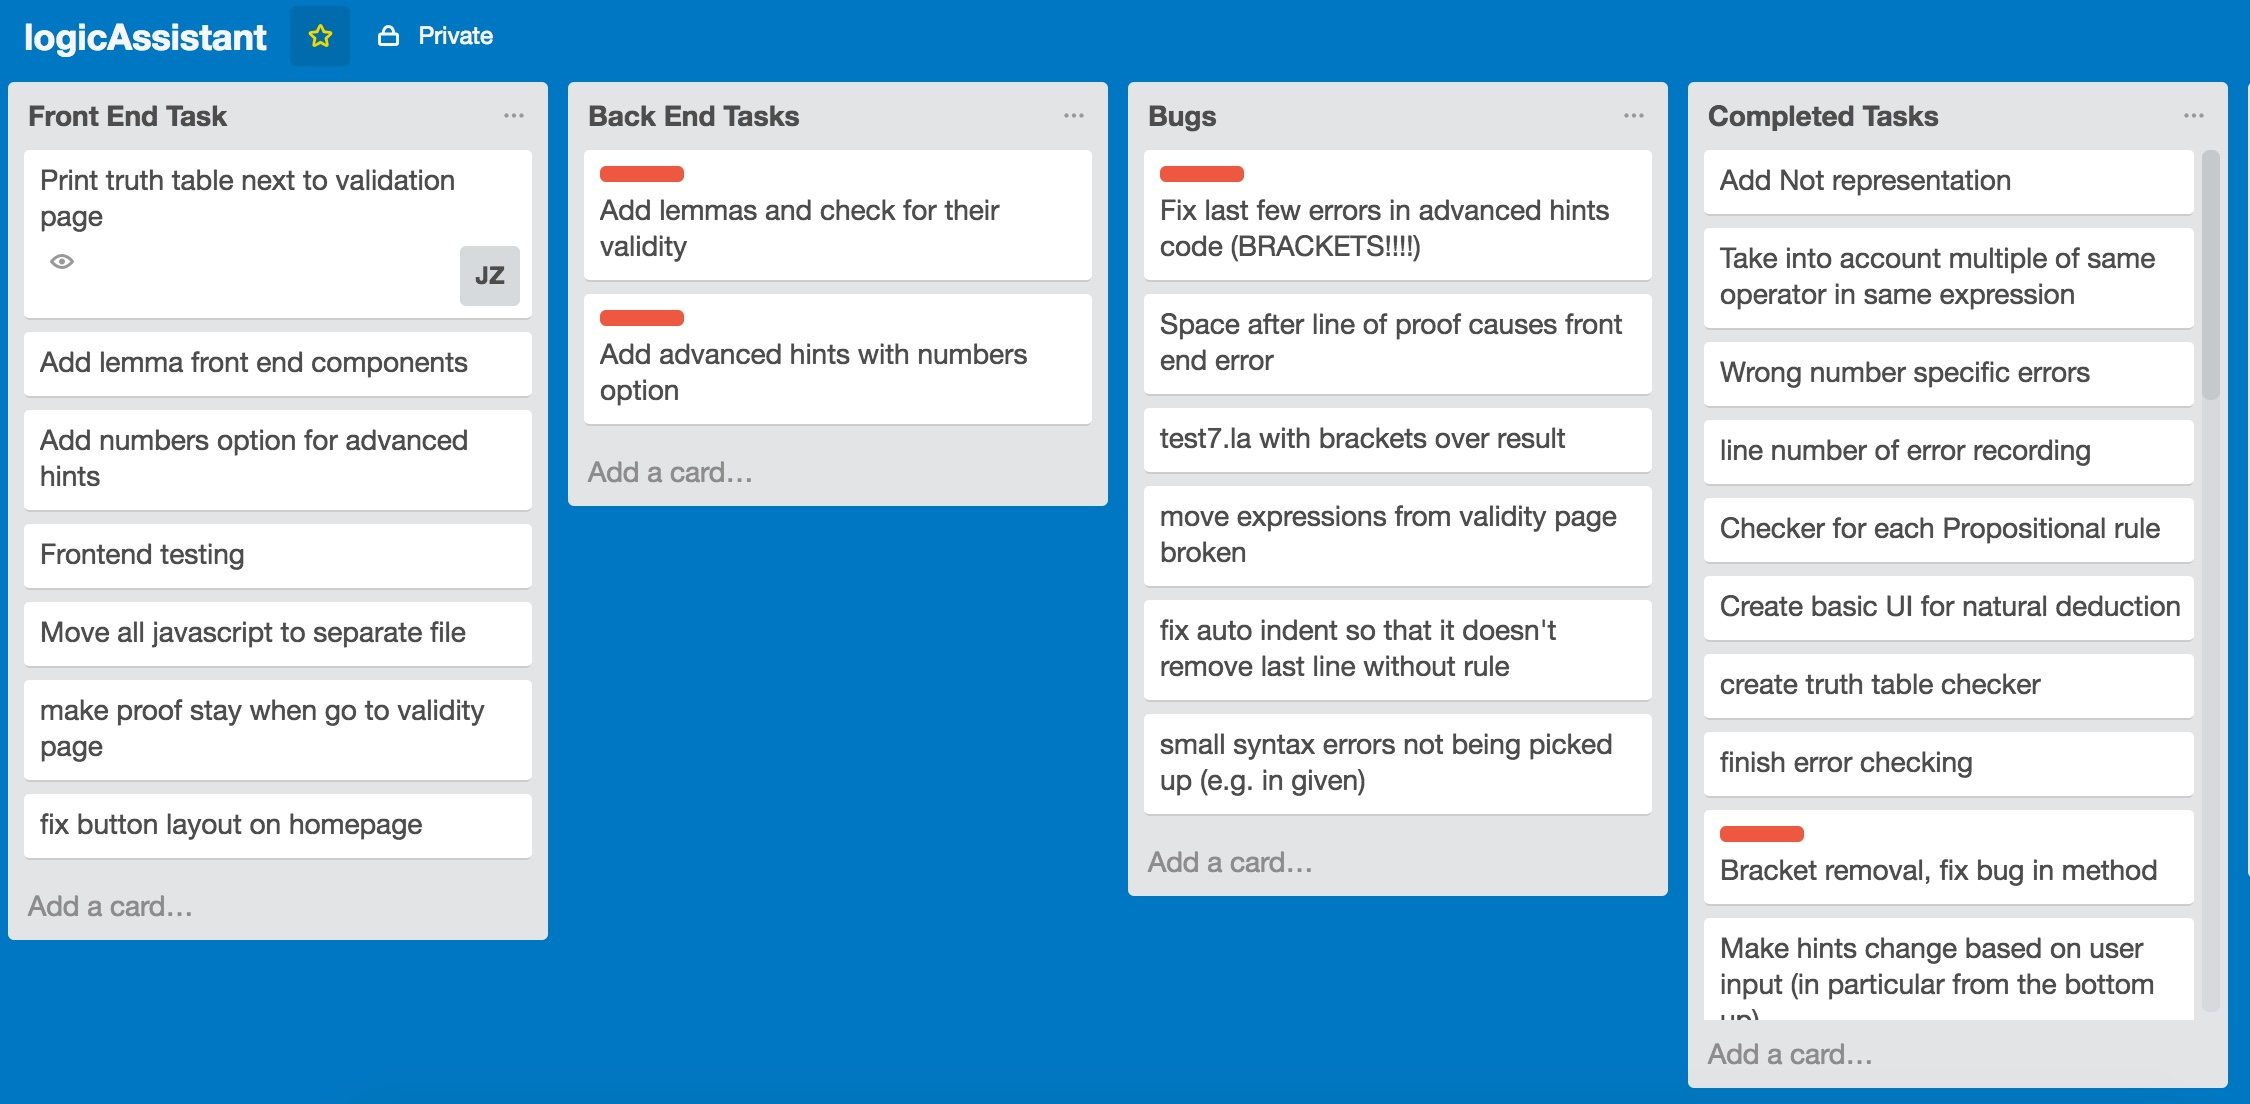
\includegraphics[width=\linewidth]{figures/trelloBoard}}
	\caption{My Trello Board}
\end{figure}

\pagebreak

\section{Evaluation}

After carrying out a large-scale project such as this, it is always good practise to evaluate how the project went as a whole. Were the objectives set out at the beginning of the project realistic? Were you able to create all of your planned functionality? Could you have avoided any set-backs that you were faced with? These ideas among others are all items to consider after having completed a project like this. By successfully evaluating a completed project, you will be able to use any lessons learnt to improve future projects.

\subsection{Realistic Objectives}

At the beginning of this project, I clearly set out several goals that I wanted to achieve by its completion (see \ref{objectives}). My main goals were to create a website that allows a user to type in their Natural Deduction proof and then using the functionality will be told whether their proof is valid. In addition to this I also planned to add hints that a user can request when they are stuck at any point of their proof. I also mentioned some extensions that time allowing, I would also like to add such as supporting Predicate logic, saving/loading of proofs and a more advanced solving algorithm for generating hints. I felt that by completing these main objectives together with some of the extensions, I would be able to create a useful Natural Deduction proof solving tool.

In the end, I was able to successfully complete the two main objectives of the project, providing the user with an easy to use interface to help them solve their Natural Deduction problems. Once I had completed these tasks I then had to decide which features were most important for me to add. In the end I decided to add the saving and loading functionality as I realised that would make the tool much easier for the user to use. I also added a validity checker based on the premises and result of a proof, so that a user can check their proof is valid before trying to solve it. Although this was not in my list of extensions, I felt that this was a very useful tool for any user. 

The biggest decision that I had to make was whether to extend the software to be able to solve Predicate logic proofs or improve the algorithm used to generate hints. Both of these tasks would have been very time consuming, so I knew I wouldn't have enough time to do both. In the end I decided to improve hint generation, for a number of reasons. Firstly, before making this decision although a basic form of hints had been created, the methodology employed was not very useful. When the user was stuck at a point in their proof and clicked the "Hint" button,  the code would just try each of the rules and see which ones were successful. It would then output to the user which rules can be used. This is of course a very short-sighted way of doing this, that could lead a user off in the completely wrong direction. I therefore decided that hints should be perfected so that they are actually helpful for the user. If I was able to generate hints that actually help point the user towards their specified goal, this tool would be a real asset for them as they learn how to solve these problems. In addition to this, before moving on to a completely new logical system such as Predicate logic, where there are lots of new areas such as quantifiers to consider, I wanted to make sure to have completely finished the functionality for Propositional logic. There would have been no point in moving on to this new logical system if the original one had not been fully implemented. I would rather there were less features created in this project that work really well than more which work less well. Once I had made this decision I ensured to design the rest of the code-base in a way that it could be easily added to if someone were to extend it to support Predicate Logic in the future. 

Overall, I was able to complete my main objectives as well as several extensions that would make the user experience better and make this tool much more useful to the user. I think that I chose wisely when it came to selecting which extensions to complete, as in the end it has lead to a website that really can help a user who is learning how to solve Natural Deduction proofs, whilst leaving the software open for further additions in the future.

\subsection{Project Plan}

At the onset of this project, I made sure to create a detailed schedule including realistic dates (see~\ref{schedule}), to plan the execution of this project. In each iteration I detailed what I wanted to achieve by its completion and how this would contribute towards the end product. The iterations themselves varied in length depending on how long I thought the various tasks would take to complete.

The first three iterations ran to plan with me easily being able to finish them by my specified deadlines. I was therefore by the end of iteration able to say that I had completed my main objectives together with an overall plan of how the rest of the project would be carried out. I had also even implemented some extra features that were not mentioned in my plans. After iteration three, I had a small break in order to revise for exams. It was at this point that, as mentioned above, I decided to no longer implement Predicate Logic, but rather a more advanced hint generation system. This meant that the subsequent iterations would be slightly different to my original plan. Iterations four to six had to therefore be merged into one as I tried to implement various proof solving algorithms and tried to solve the various bugs that I had left over from previous iterations. This was quite an intense period, but by the end I was able to complete this task. 

Although I was able to complete the tasks that I in the end decided to implement, because I changed my mind in the middle of the project, the project became a bit disorganised. From iteration four onwards I had no set plan of how to implement the remaining functionality which meant it was often difficult to decide what to do next. Trello (see \ref{trello}) was able to help me with this, but it still meant me wasting time trying to work out what to do next. It would have been best, one could say, for me to have planned exactly what I was going to implement at the beginning of the project. On the other hand however, it was only once I had properly started to create the main features of the software that I became aware of the choices that I would have to make due to time constraints. Before starting the project it was very difficult to estimate how long tasks would take, so I made some rough estimations when making the schedule. It was only once I actually started using this schedule that compromises had to be made. Therefore you could say I had no choice but to continue working without a plan. Although this was a small setback, I was able to complete all of the tasks that I in the end decided were necessary.

Overall, although I chose to change the direction of the project midway, I was able to complete the tasks that I decided to implement throughout this project. As a result of this I was not able to completely keep to the schedule that was set out at the beginning and should have changed the plans accordingly before continuing on with iteration four. This would have made it much easier for me to know which tasks to complete when, as I came towards the end of the project. I was however able to end of the project with iteration seven, where I could tidy up and finish the last parts of the important functionality that this software provides.

\subsection{Testing}
As mentioned previously (see \ref{testing}), testing was a key component of this project. I used Test Driven Development whilst developing the back-end of the system to ensure that all parts of the system were working well as new features were added. This led to a large test-suite being created. I also created several front-end test cases which simulate and test the actual functionality that a user would utilise in order to access their required features. All of this testing greatly helped towards the development of this project.

Although I was able to keep up the use of Test Driven Development for the back-end of the project, one could say that the amount of tests created in this area was a bit low. The test-suite checks most of the basic cases for the various features as well as some of the edge cases. However, more testing could have been done for the edge cases, in order to ensure that this software works in every case. As well as this, testing was mainly carried out on relatively short proofs. This means that during the project large proofs either had to be manually tested or just assumed to work based on the smaller proof tests passing. The main reason for this was due to time constraints. Writing tests for larger proofs is very time consuming and I decided to create a large number of smaller tests, which cover most of the edge cases I could think of instead. If more time was available I would spend the time adding a lot more complex test-cases to the test-suite, thereby increasing the completeness of the software.

Another missed opportunity that I had regarding the testing of this project, was when it came to the front-end. It was only quite late into the project that I decided to add these tests, because it took me a while to find an effective way to create them. But once I had created one successfully, I was able to easily add several more. Due to the time it took for me to work out an easy way to do this, it was not until midway through the project that I actually carried this out. This meant that in order to test the front-end of the software, I had to manually keep redeploying it. This was quite a time consuming process. Had I started to develop these tests earlier I would have been able to use them to help me with the development process itself. When I had eventually created these tests I ended up deciding not to create that many of them for a number of reasons. Firstly most of the functionality had already been tested in the back-end and so had been proven to work in a lot of cases. Also the time it takes to run one of these tests is a few seconds, as they actually load the web-page and perform click and input events. This meant the test-suite as a whole would take minutes rather than seconds. It would therefore be very time consuming for me to run this test suite every time a change was made. I therefore decided to have only a limited number of these tests to prove that the general features of the front-end of this application are functioning properly.

Before starting this project, as I had done in previous projects, I considered using Continuous Integration to constantly manage the test-suite for my project. This would allow me to keep constant track of my tests and would alert me if any of them fail when subsequent features are added. This can be a very helpful tool when conducting a software project with a large set of tests like this. However, in the end I decided that I would not use a Continuous Integration tool. The main reason for this was the number of other tools that I would be using that constantly alert me to whether all of my tests are passing. Firstly, by using Intellij (see \ref{intellij}), I was provided with an easy-to-use interface for running lots of test-cases with just the click of a button. This made it easy to just run specific test-cases after a piece of code has been changed. Also by using Maven (see \ref{maven}), and in particular git hooks (see \ref{git}), I was able to run all of my tests before any changes were pushed to git, thereby ensuring that all of my code was functioning correctly. Based on the use of these two technologies, I felt that I would always be kept up to date of the health of my code, and therefore the use of Continuous Development would be unnecessary.

In summary, the testing carried out on this project was relatively thorough in the back-end, but could have been improved through an increase in testing of longer and more complex proofs. In the front-end, more tests could have been added but a balance had to be maintained between the rigour of testing and the time they take to run. I also still agree with the premise that Continuous Integration was not necessary for this project. Despite some small short-falls, I feel that the testing I carried out throughout this project, greatly assisted me in its development into this completed product.

\subsection{Front-End Design}

One of the most important parts of LogicAssistant is the front-end user interface. This is the component of the application which the users themselves will be using to access its useful features, and therefore must look as good as possible. As well as being aesthetically pleasing, the front-end must also boast features which are easy to use and could be used by anyone. I therefore put a lot of thought into how I was to design the front-end of the application.

Looking back at the end design of this application, a few points can be made. Firstly, I think that the application has been created with an interface that is very easy to use. As soon as you arrive at the website you are immediately provided with the main functionality of the website, and it is immediately clear as to what the user needs to do first. All buttons are clearly labelled, with tooltips explaining certain features. This overall functionality is also quite simplistic, so that any user, no matter what their level of knowledge of this subject is, can use this application. The presence of a detailed user guide on the website also ensures that the website is as user friendly as possible. The ease of use of the user interface therefore mirrors the amount of time spent perfecting it. However, despite the large amount of time spent perfecting the front-end usability, one could argue that the design itself could be improved. When designing the website I used a very basic Bootstrap template. The reason I did this is that I felt it would be easy to add additional features to the web-page without too much of a hassle. It would also be very easy for me to make these extra features look good on the page. The entire design of the web-page could have been improved by using a better looking template in the first place. This would have made the user experience on the website even better, as it is often the design of a website that draws people into using its features. If I had more time to work on this project, this would definitely be a part of the project that I would redo, giving the web-page that slightly better aesthetic appeal.

The front-end design of this application has been created to be easy to use for users, and looks good enough to be released as a functioning website. However the overall design could still be improved, giving users an attractive website that helps them with all of their Natural Deduction proof solving needs.

\subsection{Difficulties \label{difficulties}}

Throughout my implementation of this project I was faced with a number of difficulties which hindered my overall progress. In order to solve them I had to spend large amounts of time either searching for an innovative solution or debugging the code trying to find the route of the problem. In the end I was able to fix most of these difficulties, but a large amount of time was spent trying to solve them.

\subsubsection{Algorithm Implementation}
One of the main difficulties that I was faced with, was when implementing the proof solving algorithm in order to generate hints. As mentioned above (see \ref{hints}), in order to generate hints for the user I implemented a proof solving algorithm to solve the proof and then based on this result generate a hint. The first problem with this was that the algorithm that I used, specified some of the Natural Deduction rules differently to how I specified them in this project. For example, for "Or Elimination", the following formation was used:

	\begin{figure}[!ht]
		\centering
	\begin{bprooftree}
		\AxiomC{$A \vee B$}
		\AxiomC{$\neg A$}
		\BinaryInfC{$B$}
	\end{bprooftree}
	\end{figure}

 On top of this, some rules were completely missed out of the algorithm such as all of the "Only" rules. In order to add in the missed out rules, it was not too difficult as they followed a similar pattern to other rules. However, when it came to adding "Or Elimination", I had to think of a completely different method to apply this rule. This took me a very long time to perfect, wasting other time that I could have spent on adding extra features. One could argue that due to the difficulties associated with this algorithm, it may have been more beneficial for me to have used another algorithm completely. I decided not to do this because I realised that if I was able to solve these issues, I would be able to create a very efficient way to generate hints for the user. The benefits definitely outweighed the costs, and I decided to stick with it. I was eventually able to solve these problems, thereby completing the algorithm. 

\subsubsection{Expression Bracketing}
Another difficulty that I was faced with towards the beginning of this project was the handling of brackets within expressions. Brackets are a key part of any logical expression, as they express the order of interpretation. Without the use of brackets, expressions can end up being very vague and inexpressive. In order to create a useful logical tool I therefore had to ensure that brackets could be used effectively. The first issue that I had with this was making my parser search for bracketed parts of expressions and then evaluate them in the correct order. This was especially difficult for large expressions where several sets of brackets are included. Once I had implemented this in an effective way, my next issue which which I spent a large amount of time on was "ConcurrentModification" exceptions. As my expressions are represented by lists of components, when any operation is done on the list whilst iterating through it, this exception will be thrown. This meant that I had to find inventive ways to perform these operations. This problem was very hard to debug and I dedicated a large amount of time trying to solve it. At the time of writing this report, I have not been able to fully fix this problem, but I intend to spend some time before the deadline of this project looking into ways to fix it. This will mean that any expression will be able to be successfully represented in my internal representation of Propositional Logic. This will make this project a really useful tool for Natural Deduction proof solvers.

\subsubsection{Learning Java Spring}
As mentioned above (see \ref{JavaSpring}), I used Java Spring to implement a Model View Controller architecture for this project. Although this framework gave me a concrete structure to design the project with, alongside it came some challenges. Before this project I had never used Java Spring, so the learning curve was very steep from the outset. It took me a while to fully understand how the controllers in Java Spring can be used to pass objects from the back-end to the front-end of the application, and how to navigate between web-pages using these controllers. Also, using Thymeleaf for the front-end of the Java Spring functionality brought with it further challenges. Firstly, the way I was used to using HTML and Javascript was completely changed with small nuances that had to be added in order for the page to even function. For example, in order to include Javascript and Bootstrap in the webpage itself, extra lines of code must be written in order to alert Thymeleaf to this fact. This took me a long time to get completely right, thereby hindering my front-end development process. The next huge challenge was actually recording user input into the fields of a Java object and to then apply various Java methods on them. Again with Thymeleaf comes a whole set of extra functionality with its own specific specifications that I had to learn in order to create features that meet my specification. The difficulty I found with this often meant I had to compromise on the front-end aesthetics in order for me to create my required functionality. One of the main reasons why I found this tool so difficult to use, was the fact that there is very little helpful information online. In contrast to Java itself, which has a wealth of information online, Java Spring's online content is quite sparse and was therefore not able to help me very much. It took me a long time to find help for specific problems I was having, and the tutorials could only help me so far to solve them. It therefore took me a very long time to get used to using this framework, but the benefits it provided me with as a whole made it an asset to this projects' development. By the end of this project, after having struggled through learning how to use Java Spring's core features, I have now learnt how to use it effectively for future web based projects.

These difficulties are some of the many difficulties that I was faced with as I went through this project. Some involved me spending large amounts of time working on them in order for me to solve the associated problem, and some may have even been avoided had I used alternative technologies. However, I was in the end able to work through most of them allowing me to in the end deliver this finished product. All the difficulties I faced taught me many lessons that I can take away from this project, that I can apply to future similar problems that I may be faced with in my future career. 

\subsection{Competitor Analysis}

The main competitor to LogicAssistant, based on its use as an assistant to solve Natural Deduction proofs and as a learning tool, is Pandora. Pandora was created at Imperial College London \cite{pandora}, as a tool to assist students as they learn how to solve Natural Deduction proofs. Pandora differs from LogicAssistant in a number of different ways, making it an arguably better tool than Pandora. A comparison between these two tools is discussed in this section.

The first main difference between LogicAssistant and Pandora is the type of software offered. Pandora is a Java Application which must be installed on a computer in order to be used. In addition, this software assumes that Java has been installed on the computer before Pandora can be executed. The process of setting up Pandora is different on each operating system, and will not function unless configured correctly. LogicAssistant on the other hand, is fully web based. I have tested to ensure that the website functions properly on all of the main web browsers and operating systems, so it is almost guaranteed to work on whatever setup you are using. All the user needs to do is go to the LogicAssistant URL, and they are immediately provided with all of this useful functionality. The one drawback of the LogicAssistant setup, is that if a user does not have internet access they will not be able to access this service, whereas they would still be able to use Pandora. However, nowadays one can assume that most people do have consistent internet access, so will be able to use this service whenever they like. Another benefit of having the software on a web platform, is that it can be accessed from other devices such as phones or tablets. LogicAssistant can therefore be used by users who only have a phone or tablet to hand, wherever they are, when they are trying to solve some Natural Deduction Proofs. This is in contrast to Pandora which due to it being a Java application must be used on a computer or laptop.

There are two important features that are provided by Pandora which can seem to be quite annoying for the user. Firstly, when Pandora is first opened in order to start writing a proof, the premises and resulting expression must be typed in. Then before the proof can be started these expressions are checked to see whether a proof using them would be valid. This means that someone learning how to solve these proofs can't even attempt the proof, in order to learn from their mistakes, before being told that they are doing something wrong. As well as this, once a proof has been started, a user can only enter a line into the proof if it is valid. Both of these features make Pandora a hard tool to use for someone learning how to solve these proofs. It would be much more educational for the user to actually type in their ideas for a proof and then for the software to tell them what they have done wrong. The reason for these "problems", could be that Pandora was designed with different objectives, helping the more advanced users check their proofs. The functionality provided therefore will be at the right level for these users.  LogicAssistant however, has an additional objective of being an educational tool for users of all levels and was therefore built without this features. This means LogicAssistant allows the user to type their entire proof into the text boxes first, before checking whether each step is valid. This allows a user to slowly learn from any mistakes they have made. There is an option for the user, if they choose, to check the validity of their proof at any point, but it is their choice whether to do this or not. This extra freedom makes LogicAssistant a really useful learning tool for these proofs. 

One of the parts of Pandora that I believe is still much better than LogicAssistant, is how boxes (new scopes) are displayed in a proof. In LogicAssistant when a new scope is entered, in order to emphasise this, the lines are indented and indicated by four minus signs. This indentation increases if subsequent boxes are later entered. Although this does indicate to the user that a new scope has been entered, it is not that aesthetically pleasing. Pandora is much better at representing this, as it actually draws a box around any expressions which are in a different scope, clearly notifying the user to this fact. This makes the entire proof much more readable for the user, and thereby more understandable for any new users of this proof system. If I were to have more time to spend improving LogicAssistant, I would try to implement similar details to its front-end. This would allow users to really get the most from this educational tool. 

The main additional feature that LogicAssitant provides, is the generation of hints. If a user becomes stuck while using Pandora at any point in their proof, they will have to stop and try to work out a solution for themselves. They may even be forced to start again in order to try to find a better direction to go in. LogicAssistant on the other hand is able to help users who are faced with this problem. If a user is stuck at any point of the proof, whether they are in the middle of a proof and are not sure what step to carry out next, or if they have steps missing in their proof, LogicAssistant can provide them with the hints needed for them to continue. LogicAssistant doesn't tell them the answer, as this would defeat the educational purpose of the tool. Rather it gives a hint as to what the next rule in the proof should be. This then helps the user to move further into the proof, happy in the knowledge that they are going in the right direction. LogicAssistant is therefore much more helpful for a user as they start to learn how to solve Natural Deduction Proofs.

One of the key features of both of these tools which make them really useful as educational tools, is error message generation. Both tools provide error message whenever a syntax error is made or when a rule has been used wrongly. With regards to syntax errors, I think that both tools equally provide useful and informative error messages that assists a user as they are trying to work out where they have gone wrong. It is with regards to the other types of errors however, that the two tools differ. With Pandora if a user tries to use a rule incorrectly an error message will be generated. This error message usually just says that this rule cannot be used here without any specific reason for this. The user then must apply their knowledge of the Natural Deduction rules to this case, in order to realise what they have done wrong. This means that a user needs at least a basic knowledge of this area before being able to use Pandora's full functionality. LogicAssistant on the other hand, builds upon this type of error giving the user much more information. Whenever a Natural Deduction rule is used incorrectly in LogicAssistant a Rule error is generated. This type of error tells the user what lines the error has occurred on as well as some extra information about why this error has been thrown. Whether an incorrect line has been referenced or the rule can't be used on this expression due to the operators it contains, the user will be notified to this fact. This means that they will instantly know where they have gone wrong, will learn from their mistake and be able to move on with the proof. This again shows us another important educational feature that LogicAssistant provides in a much more useful way than Pandora.

Finally, Pandora has several more advanced features which are currently missing from LogicAssistant. For example, Pandora supports proofs that are written using First Order Predicate Logic, including all of the associated Natural Deduction rules. It also includes some other useful rules such as Proof by Contradiction which help to keep proofs concise. Another really useful feature employed by Pandora is "Undo" and "Redo" buttons. These buttons make it really easy to undo or redo any parts of a proof that a user may have done incorrectly. This makes the entire proof writing experience much easier. These features and more are currently lacking in LogicAssistant, and with more time would definitely be on the agenda to be implemented.

To conclude, both LogicAssistant and Pandora are useful tools for anyone learning how to solve Natural Deduction Proofs. Pandora contains lots of advanced features and a nice looking display of proofs, but is lacking in ease of use meaning it is not always helpful for a stuck user. LogicAssistant, although lacking in some of the features that Pandora provides, encompasses features that make it really useful for almost any user learning how to solve Natural Deduction Proofs. Whether its the detailed error messages, hints or other useful features, a user will never be stuck in the middle of a proof not knowing what to do. This is one of the main reasons LogicAssistant was built, to provide an educational proof solving tool that solves the many shortcomings of similar proof solving software.

\subsection{User Feedback \label{feedback}}

One of the best ways to judge how well my project is going is by gaining some user feedback. This feedback will give me a window into the minds of potential users, helping me to improve the overall user experience. In order to gain some user feedback, I carried out a survey at the beginning of June, using the current stable version of the website. I used SurveyCrest (see \cite{surveyCrest}) to create a survey containing some questions in important areas of the project that I wanted feedback on. This survey can be seen in Appendix \ref{appendix:surveyCrest}. In order to gain data from this survey, I personally met with fifteen people to show them what LogicAssistant has to offer and let them try it out for themselves. Of the people I surveyed ten were Computing students who were well versed in Natural Deduction practises, while the other other five had a very basic knowledge of Natural Deduction but had never studied it in detail. After they had tried out the various features I asked them to fill out a survey. The survey contained questions first finding out the users background in Natural Deduction, then asking about how they found using LogicAssistant, what features were good and bad and finally whether they liked the user interfaces design. I used a lot of the data gathered to further improve my project.

Looking at the results of the survey a number of conclusions can be drawn, some of which I worked on in order to improve the overall product. Firstly of those surveyed 60\% of users already use some kind of tool to help them with their Natural Deduction proofs. LogicAssistant for these people is therefore a competing product, which I will have to prove to be superior to the ones they are currently using. For the rest of the people surveyed, LogicAssistant will need to show these people the benefits of using such a tool, especially how it will make the entire proof solving process much simpler. Another question that was asked in the survey was how LogicAssistant compares to other similar products that those surveyed had used. All of them replied that it was at least slightly better than other software they had experienced. This showed me that LogicAssistant must be doing something right, especially as even those who don't commonly use this type of software support its achievements.

One of the main goals that I wanted to achieve by the end of this project was to make this application as easy to use as possible. This would allow LogicAssistant to attract users at lots of different levels of knowledge of Natural Deduction, as they try to solve their complex proofs. In order to test how successfully I had done this, I asked in the survey for people to rate how easy to use LogicAssistant was out of ten. The results can be seen on the graph below. This graph shows how all of the people surveyed thought that the website was relatively easy to use. In another of the survey questions I asked what is missing from this tool as a whole. Several people answered that it was a bit difficult to figure out exactly what to do upon arriving at the website. They especially said this regarding the hints option. In response to these comments I made sure to make it very clear using extra tooltips and by making some of the features more simple, exactly how to use the application. I would hope that the finished product today now has resolved these issues and is therefore very easy for any user to use.

\begin{figure}[!ht]
	\centering
	\makebox[\textwidth]{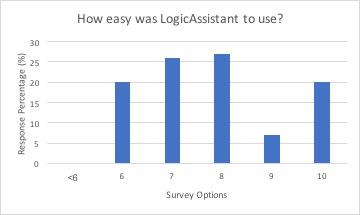
\includegraphics[width=13cm]{figures/easeOfUseGraph}}
	\caption{Ease of use survey results}
\end{figure}

Another key component that I wanted to gain feedback on, was the design of the front-end of the application. This is the part of the application that the users will actually see, so must be aesthetically pleasing as well as having features that are displayed clearly. I again asked the people I surveyed to rate how they find the design of the user interface. The results of this question can be seen on the graph below. This graph similarly shows that most people surveyed thought the design of the website was quite good as well as just being easy to use. A few gave a slightly lower score, and in answering what is missing from this application they say that how the proof itself is displayed is a bit lacking. They add it would be nice to have proper boxes around new scopes, as well as more of a notification when a proof is found to be valid. I did not in the end have time to work on these constructive points, but these items would definitely be on the agenda to implement next if I was to continue working on this project. 

\begin{figure}[!ht]
	\centering
	\makebox[\textwidth]{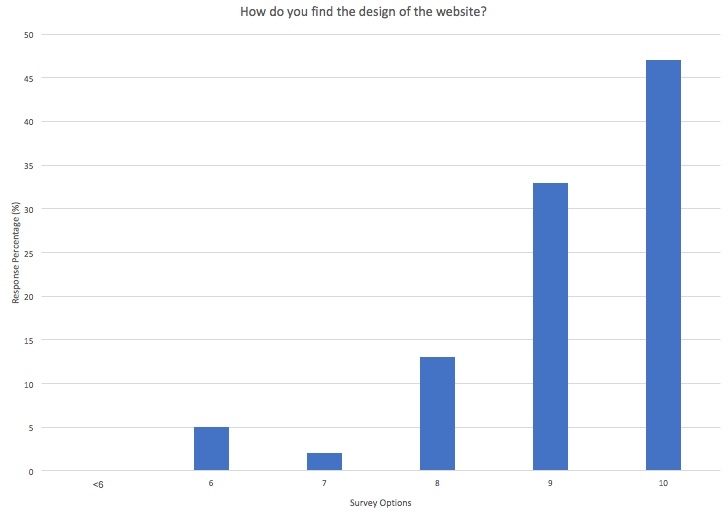
\includegraphics[width=13cm]{figures/websiteDesignGraph}}
	\caption{Website Design survey results}
\end{figure}

In order to see whether the features that I had implemented were demanded by potential users, I also asked people which features were most important for this tool to have. A majority of those surveyed answered that hints were the most important, and are a fundamental tool to have on an application such as this. Other important features that were mentioned were the validation of proofs and having a clear user interface. These results show me that users recognise how useful the various features provided are for solving these problems. As mentioned above I also asked which features users thought were missing from LogicAssistant. As well as an increase in user help, which I made sure to work on, users suggested support for Predicate Logic and the addition of undo and redo buttons to the user interface. As mentioned many times in this report the addition of Predicate Logic to this tool was not included due to time restraints. If more time was on offer this would definitely be an extension that could be added to this application. Similarly, redo and undo buttons could be easily added in the future. These were the main places where users felt this software was lacking.

The user feedback that I gained provided me with invaluable information about my application as a whole. However, the way I carried out the retrieval of this feedback could have been improved in several ways. Firstly, I left it very late on in the project before I carried out this survey, meaning that there was only so much I could do in the remaining time to work on the feedback that I gained. It would have been much more useful to have done this towards the middle of the project where I could use the data gained to ensure that the project was heading in the right direction. In addition to this, it would have been helpful if I had asked a bigger range of people to answer my survey. Not just by asking more people but people with a whole spread of different knowledge levels of the topic of Natural Deduction. This would have given me an even clearer picture of how my tool can help the needs of each of those ability levels. Finally, I could have also included a larger number of questions in the survey to find out even more information about my application. I could have gone into a lot more detail, and the data gained could have helped to tailor my application to the demands of users even more. By doing this I would be able to provide the best experience possible for any user.

Overall, I have conducted a survey in order to gain user feedback for my application. The data gained was very useful for me as I made the final touches to the user interface and back-end functionality. Although in several areas the way I retrieved user feedback could have been improved, in the end I was able to gain a clear image of what a user really wanted to get out of my application and which features really help them to do this. 


\pagebreak
\section{Conclusion}

LogicAssistant provides a user with a tool to check whether a Natural Deduction proof they have written using Propositional Logic is valid. In addition to this, if a user becomes stuck at any point in their proof, hint functionality is available to help the user work out which rule to apply next. These core features, together with some extensions, provide users with an educational tool to help them learn and improve their Natural Deduction proof solving skills. 

After having successfully completed this project, I can look back at the achievements and learning outcomes that I have gained. I now have a completed application that really can help people learning how to solve Natural Deduction problems work through any issues that they may have. My main objectives have been met and although I encountered some issues along the way, the project can overall be judged a success. I am very happy to have carried out this project in particular, as I was able to learn lots of different lessons about how to conduct projects in this area.

\subsection{Learning Outcomes}
This project has forced me to learn how to solve and work through complex Natural Deduction problems in a thorough way. I can now easily look at a Natural Deduction problem and without much thought be able to work through the problem. This is definitely a very useful tool to have in this field. The project has also shown me the various issues associated with the automated solving of Natural Deduction Problems. As discussed in great detail in the design section (see \ref{hints}), there are so many different cases to think about, making this a very difficult problem to solve. The algorithm that I ended up with provides an innovative way to solve these problems, and gave me a whole new way of thinking about the solving process of these proofs. 

Through the carrying out of this project, I also learnt how to successfully manage a large-scale software engineering project. The issues that I had midway as I chose to follow certain objectives (see \ref{difficulties}), taught me the importance of always having a very detailed plan at the beginning of the project. Also how big decisions such as which objectives to complete first in a project should be decided early on in order to avoid wasting time while plans are changed. In addition to this I learnt how to properly manage the task that I planned to complete ensuring that they were all completed by their specific deadline. The part of this project that went very well and has shown me how useful it is for this type of project, is the use of Test Driven Development (see \ref{testing}). Using this methodology the writing of the back-end components of the code-base became much easier and I was always able to be sure that the code-base as a whole was functioning correctly. Test Driven Development really helped me to successfully complete this project. These practises among other helped me to successfully complete this project, and are definitely techniques that I will take with me to future project.

An additional lesson that I learnt from this project was how to use a web framework like Java Spring. In the past I have mainly worked on back-end style projects and have very little experience using front-end technologies. Through the learning of how to use Java Spring I have been able to fully understand how all of the different components of the application work together to create the finished product. How the front-end is able to communicate with the back-end in order to supply the user with their required functionality and how useful a Model View Controller architecture (see~\ref{design}) is in creating a well structured and easy to read code-base. This technology is a fundamental part of building web applications, and is an important skill for me to have learnt. I will definitely use this skill as I embark on future web based projects.

Overall, through the learning of these lessons and others, I have through this project been able to improve as a software engineer. The lessons learnt will greatly assist me in future projects that I may undertake and this makes this project an important building block for my career. I can now look back at this project and see what a useful tool I have created that can assist users of all ability levels as they strive to learn how to solve Natural Deduction problems.

\subsection{Future Work}

As this project had only a limited timespan, there were a number of features that I was not able to add to the application. If I were to spend more time on this project or someone was to further extend this application, the following features would be next on the list to be added. With the addition of these features, the overall usefulness and ease-of-use of this application would be significantly increased. 

The first addition that I would like to make, which has been discussed at length throughout this report, is the addition of support for Predicate Logic. One of my initial aims that I said that time allowing I would like to complete, was the support for this more expressive logical environment. As discussed in the background section (see \ref{predicate}), Predicate logic can be used to represent expressions that are much more expressive, and the associated Natural Deduction rules build upon those of Propositional logic. These extra rules make Natural Deduction quite complex, so to have a tool which assists a user with this type of proof would be very helpful. I have created the application in a way that it can be easily built upon, so adding the Predicate representation and then rules would be relatively easy. The solving algorithm used for hints (see \ref{hints}), also supports Predicate logic, so my implementation of this algorithm can easily be adapted. By adding this feature, this application as a whole would become even more useful for people learning how to solve more complex Natural Deduction proofs.

Based on user feedback gained (see \ref{feedback}), as well as my own testing of the user interface, there are a few small features that could be added to the application that will make it much easier to use. The first very useful addition would be undo and redo buttons. Rather than a user having to retype what they deleted, these buttons would provide the user of an easy way to edit their proofs. In addition to this, at the moment a user has to physically type in the line numbers of any lines that a rule is referencing which can be quite annoying, so what would be very useful would be for the application itself to automatically add these line numbers. This is what happens in similar applications such as Pandora (see \cite{pandora}). This would make the whole process of writing proofs much simpler. These and several other small tweaks to the front-end of the application would make the user experience even better.

A further area of this application that could be improved with extra time, would be the front-end design and representation of proofs. At the moment I have created a simple template using Bootstrap (see \ref{bootstrap}), that is easy-to-use but the design itself could be improved greatly. I would spend time adding a more advanced and better looking template that would make the website look even better. It is often a good looking website that encourages users to use it, and I would therefore invest time making it look as good as possible. On top of this, based on user feedback (see \ref{feedback}), the way that new scopes in a proof are displayed would look much better using actual boxes. This would properly separate the scope from the rest of the proof, and make the proof as a whole look much tidier than the current indentation used. Also at the moment the only indication that is given that a proof is valid is a message appearing at the bottom of the screen. With extra time I would also add other indicators, such as the proof being highlighted in green to show this. With these and several other ideas, I would with time try to improve the overall design of this application.

To conclude, in order to improve and further develop this project, I would implement the above ideas among others, to advance the application as a whole. Although the application currently provides a useful tool to users, these extra additions would bring this application to a completely new level assisting even more users with their problems. LogicAssistant is therefore a fundamental tool for anyone learning how to solve Natural Deduction proofs, and with a few additions this tool will be an incredible asset to logicians worldwide.

\pagebreak
\appendix
\section{Natural Deduction Rules}
\label{appendix:nd}

\subsection{Propositional Rules (adapted from \cite{ndBook})}
\label{appendix:nd-prop}


\begin{namedthm}{Rule}[And Introduction]

\begin{bprooftree}
\AxiomC{$A$}
\AxiomC{$B$}
\BinaryInfC{$A \wedge B$}
\end{bprooftree}\qquad or \qquad
\begin{bprooftree}
\AxiomC{$A$}
\AxiomC{$B$}
\BinaryInfC{$B \wedge A$}
\end{bprooftree}

\end{namedthm}

\begin{namedthm}{Rule}[And Elimination]

\begin{bprooftree}
\AxiomC{$A \wedge B$}
\UnaryInfC{$A$}
\end{bprooftree}\qquad or \qquad
\begin{bprooftree}
\AxiomC{$A \wedge B$}
\UnaryInfC{$B$}
\end{bprooftree}

\end{namedthm}

\begin{namedthm}{Rule}[Or Introduction]

\begin{bprooftree}
\AxiomC{$A$}
\UnaryInfC{$A \vee B$}
\end{bprooftree}\qquad or \qquad
\begin{bprooftree}
\AxiomC{$A$}
\UnaryInfC{$B \vee A$}
\end{bprooftree}

\end{namedthm}

\begin{namedthm}{Rule}[Or Elimination]

\begin{bprooftree}
\AxiomC{$A \vdash C$}
\AxiomC{$B \vdash C$}
\AxiomC{$A \vee B$}
\TrinaryInfC{$C$}
\end{bprooftree}\qquad where A and B are assumptions

\end{namedthm}

\begin{namedthm}{Rule}[Not Introduction]

\begin{bprooftree}
\AxiomC{$A \vdash \bot$}
\UnaryInfC{$\neg A$}
\end{bprooftree}\qquad where A is an assumption

\end{namedthm}

\begin{namedthm}{Rule}[Not Elimination]

\begin{bprooftree}
\AxiomC{$\neg  A$}
\AxiomC{$A$}
\BinaryInfC{$\bot$}
\end{bprooftree}\qquad 

\end{namedthm}

\begin{namedthm}{Rule}[Double Not Elimination]
	
	\begin{bprooftree}
		\AxiomC{$\neg \neg A$}
		\UnaryInfC{$A$}
	\end{bprooftree}\qquad 
	
\end{namedthm}

\begin{namedthm}{Rule}[Implies Introduction]

\begin{bprooftree}
\AxiomC{$A \vdash B$}
\UnaryInfC{$A \Rightarrow B$}
\end{bprooftree}\qquad where A is an assumption

\end{namedthm}

\begin{namedthm}{Rule}[Implies Elimination]

\begin{bprooftree}
\AxiomC{$A$}
\AxiomC{$A \Rightarrow B$}
\BinaryInfC{$B$}
\end{bprooftree}\qquad 

\end{namedthm}

\begin{namedthm}{Rule}[Iff Introduction]

\begin{bprooftree}
\AxiomC{$A \Rightarrow B$}
\AxiomC{$B \Rightarrow A$}
\BinaryInfC{$A \Leftrightarrow B$}
\end{bprooftree}\qquad 

\end{namedthm}

\begin{namedthm}{Rule}[Iff Elimination]

\begin{bprooftree}
\AxiomC{$A \Leftrightarrow B$}
\UnaryInfC{$A \Rightarrow B$}
\end{bprooftree}\qquad or \qquad
\begin{bprooftree}
\AxiomC{$A \Leftrightarrow B$}
\UnaryInfC{$B \Rightarrow A$}
\end{bprooftree}

\end{namedthm}


\subsection{Predicate Rules}
\label{appendix:nd-pred}

\begin{namedthm}{Rule}[$\forall$ Introduction]

\begin{bprooftree}
\AxiomC{$P(a)$}
\UnaryInfC{$\forall x.P(x)$}
\end{bprooftree}\qquad where a is arbitrary \qquad

\end{namedthm}

\begin{namedthm}{Rule}[$\forall$ Elimination]

\begin{bprooftree}
\AxiomC{$\forall x.P(x)$}
\UnaryInfC{$P(a)$}
\end{bprooftree}\qquad where a is arbitrary \qquad

\end{namedthm}


\begin{namedthm}{Rule}[$\exists$ Introduction]

\begin{bprooftree}
\AxiomC{$\exists x.P(x)$}
\AxiomC{$\forall x.(P(x) \Rightarrow Q)$}
\BinaryInfC{$Q$}
\end{bprooftree}\qquad

\end{namedthm}

\begin{namedthm}{Rule}[$\exists$ Elimination]

\begin{bprooftree}
\AxiomC{$P(t)$}
\UnaryInfC{$\exists x.P(x)$}
\end{bprooftree}\qquad where t is any term

\end{namedthm}

\begin{namedthm}{Rule}[Substitution]

\begin{bprooftree}
\AxiomC{$m = n$}
\AxiomC{$S(n)$}
\BinaryInfC{$S[m/n]$}
\end{bprooftree}\qquad or \qquad
\begin{bprooftree}
\AxiomC{$m = n$}
\AxiomC{$S(m)$}
\BinaryInfC{$S[n/m]$}
\end{bprooftree}

\end{namedthm}

\pagebreak

\section{User Guide}
 \label{appendix:userGuide}
 
To be created

\pagebreak

 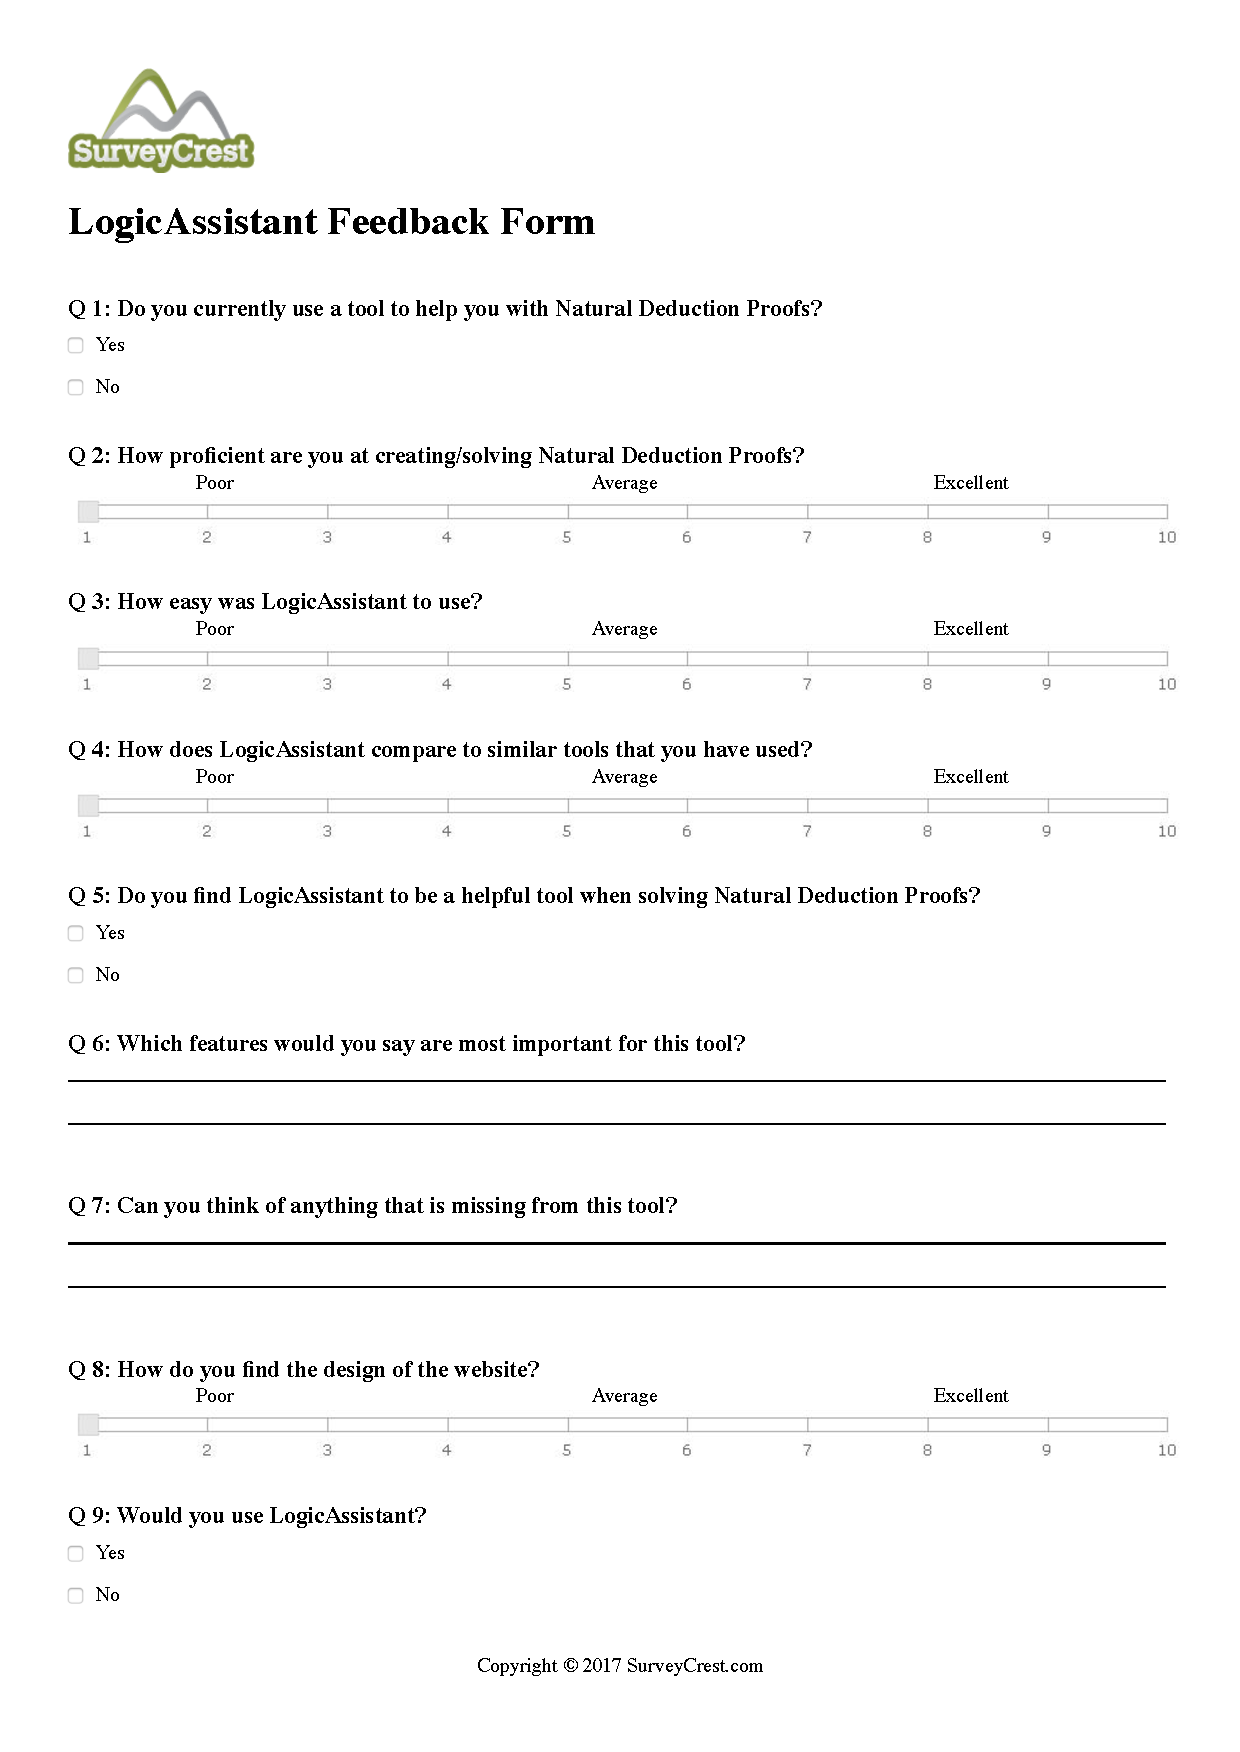
\includepdf[scale=0.75,pagecommand=\section{User Survey \cite{surveyCrest}}]{figures/SurveyApplication.pdf}
 \label{appendix:surveyCrest}

\begin{thebibliography}{9}

\bibitem{pandora} 
Pandora (Proof Assistant for Natural Deduction using Organised Rectangular Areas) is a learning support tool designed to guide the construction of natural deduction proofs. Found at \url{https://www.doc.ic.ac.uk/pandora/}, last retrieved 7/2/2017

\bibitem{ndBook}
Software Engineering Mathematics by Jim Woodcock and Martin Loomes, 1989 edition

\bibitem{ndAlgo}
Alexander Bolotov, Vyacheslav Bocharov, Alexander Gorchakov, Vasilyi Shangin \textit{Automated First Order Natural Deduction}. Conference Paper, January 2005

\bibitem{surveyCrest}
SurveyCrest, Free online survey creator. Found at \url{ https://www.surveycrest.com/}, last retrieved 6/6/2017


\end{thebibliography}



\end{document}
